\documentclass[12pt]{article}

\usepackage{amsfonts,amssymb,amsmath}
\usepackage{setspace,achicago,graphicx}

%for avoiding figures going anywhere
\usepackage{placeins}

\usepackage{hyperref}

\newtheorem{lemma}{Lemma}
\newtheorem{assumption}{Assumption}
\newtheorem{proposition}{Proposition}
\newtheorem{definition}{Definition}
\newenvironment{proof}[1][Proof]{\noindent \textbf{#1.} }{\  \rule{0.5em}{0.5em}}

\usepackage[top=.9in, bottom=.9in, left=.9in , right=.9in,letterpaper]{geometry}

%for nice caption in table
\usepackage{caption}
\captionsetup[table]{skip=5pt}

%For accepting graphs
\usepackage{graphicx}


%%%%%%%%%%%%%%%%%%%%%%%%%%%%%%%%%%%%%%%%%%%%%%%%%%%%%%
%Other Packages%%%%%%%%%%%%%%%%%%%%%%%%%%%%%%%%%%%%%%%
%%%%%%%%%%%%%%%%%%%%%%%%%%%%%%%%%%%%%%%%%%%%%%%%%%%%%%


%Within Document References
%\usepackage[colorlinks]{hyperref}
%\usepackage[colorinlistoftodos]{todonotes}
%\usepackage[colorlinks]{hyperref}
%\usepackage[nameinlink,capitalize,noabbrev]{cleveref}

%\hypersetup{
%	colorlinks,
%	linkcolor={blue!50!black},
%	citecolor={blue!50!black},
%	urlcolor={blue!80!black}}



%%%%%%%%%%%%%%%%%%%%%%%%%%%%%%%%%%%%%%%%%%%%%%%%%%%%%%
%%%%%%%%%%%%%%%%%%%%%%%%%%%%%%%%%%%%%%%%%%%%%%%%%%%%%%
\parskip3mm\parindent0cm


\title{Catholic Censorship and the Demise of Knowledge Production in Early Modern Italy}
\author{Fabio Blasutto \and David de la Croix$^2$}



\begin{document}
\maketitle


\begin{abstract}
Censorship makes new ideas less available to others, but also reduces the share of people choosing a non-compliant activity. 
We propose a new method to measure the effect of censorship on knowledge growth,  accounting for $i)$ endogenous selection of agents into compliant vs non-compliant ideas $ii)$ endogenous timing of censorship, which depends on the expected growth of non-compliant ideas. 
We apply our method to the censorship by the Catholic Church of books written by members of Italian universities and academies over the period 1400-1750.
We highlight two new facts: $i)$ once censorship was introduced, censored authors were of better quality than the non-censored authors, but this gap shrunk over time $ii)$ the intensity of censorship decreased over time. These facts are used to identify the deep parameters of a model linking censorhip to knowledge diffusion and occupational choice. We conclude that censorship explained x\% of the decline in total publications per scholar in Italy. Endogenizing censorship itself, we also show that even if the Church was bound to loose against non-conformist ideas in the long-run, censoring might still be worthwhile temporarily to delay its demise.\\
\mbox{ }\\
JEL Classification Numbers: \\
Keywords:
\end{abstract}

\footnotetext[1]{IRES/LIDAM, UCLouvain \& National Fund for Scientific Research (Belgium). Email: fabio.blasutto@uclouvain.be}
\footnotetext[2]{IRES/LIDAM, UCLouvain \& CEPR. Email: david.delacroix@uclouvain.be.\\
\indent This project has received funding from the European Research Council (ERC) under the European Union's Horizon 2020 research and innovation programme, under grant agreement No 883033 “Did elite human capital trigger the rise of the West? Insights from a new database of European scholars.”}

\thispagestyle{empty}
\newpage
\onehalfspacing

\section{Introduction}
Italy's primacy in knowledge creation was undisputed in the fifteenth and sixteenth century. Yet, it was overtaken by North and Western Europe in the following two centuries, during which scholars and the knowledge they produced are believed to have played an important role in the Rise of the West \cite{mokyr2016}. The first candidate to explain such a reversal of fortune is the fight led by the Catholic church against novel ideas \cite{land99}. These novel ideas were at the root of the scientific revolution in Europe. What is the role of the Catholic Church for the demise of knowledge production in early modern Italy?

This paper tackles this issue by focusing on the role of one weapon in the church arsenal, namely the power to censor books published by scholars. The list of such prohibited books is called {\em Index Librorum Prohibitorum}. The question we address is whether such censorship was key in altering the growth path of the generation of new knowledge in the Italian peninsula.

We answer the question with three contributions. First, we build a database of scholars active in Italy from 1400 to 1750, highlight two new facts: $i)$ once censorship was introduced, censored authors were of better quality than the non-censored authors, but this gap shrunk over time $ii)$ the intensity of censorship decreased over time. Second, we use these facts to identify the deep parameters of a novel model linking censorship to knowledge diffusion and occupational choice. Third, we perform a counterfactual experiment to asses quantitatively the role of the censorship on the decline in total publications per scholar in Italy. The use of the estimated model to evaluate the impact of censorship results in a new method which accounts for $i)$ endogenous selection of agents into compliant vs non-compliant ideas $ii)$ endogenous timing of censorship. Thus, this paper consists of three parts, one for each contribution, which we now describe in more detail.


In the first part of the paper we build a database of Italian scholars active in the renaissance academies and universities from 1400 to 1750. For each scholar, we identify whether his (or her) work was subject to censorship by the church. We also measure the ``quality'' of each scholar by the quantity of written output by him or her in the library catalogues of today. Using this new database, we document the drop in publications per person over the period 1400-1750. Studying the distribution of the publications per person, we highlight two novel  patterns. $i)$ In the sixteenth century, the censored authors are of much better quality, on average, than the non censored authors. Moreover, this difference shrinks over time. $ii)$ The intensity of censorship decreases after it was first introduced in the sixteenth century.

In the second part of the paper, we design a structural model linking censorship to knowledge diffusion. In the model, knowledge is codified in books and can be of two types: conformist and non-conformist. Following the literature on knowledge diffusion \cite{lucas2009,lucas2014}, we assume that authors randomly draw ideas from the stock of knowledge left by the previous generation, retaining the best one. We introduce a novel occupational choice to be made by printers between printing compliant / conformist books or revolutionary / non-conformist books. Hence, revolutionary books are less likely to be printed if they are of lower quality or if they are more rare than compliant books.\footnote{In a robustness of the model we also consider the possibility that authors and printers self-censor because of the fear of being persecuted by the Inquisition.} We show that, by censoring revolutionary books, the Church can not only reduce the share of people in the revolutionary occupation, but, more importantly, alter drastically the development path of knowledge. An initial temporary blow to the revolutionary ideas can force convergence of the society towards a compliant steady state. Since setting up a censorship apparatus is costly, if the Church displays impatiance, she has the incentive to delay censorship. This rationalizes why the Church waited several decades after the rise of Protestantism before starting to censor heretic books.

% We introduce a novel occupational choice to be made by scholars between developing compliant / conformist ideas or revolutionary / non-conformist ideas.

In the third and last part of the paper, we use the facts highlighted in the first part to identify the deep parameters of the structural model. The most important parameter, namely the rate of censorship, is intuitively identified by the growth of the share of censored authors. The model implies a one-to-one relationship between the share of censored authors and the relative quality of the two sectors, conditional on parameter values. Hence, the ability of the model to also match the (targeted) dynamics of the overall quality and that of censored authors support the mechanisms that we propose.\footnote{It is not possible to directly target the relative quality in the two sectors since we cannot observe authors who are both non-censored and non-compliant. The quality of non-censored authors is left as an over-identification check. The fit of this moment ``quality'' the model assumption that the quality of censored and non-censored heretic authors is the same.} The fixed cost necessary to impose censorship is picked to match the timing of the creation of the first index of forbidden books. Simulations shows that imposing a censorship rate of x\% on the non-conformist books was sufficient to decrease the share of non-conformist authors from y\% in 1550 to z\% in 1650. This impacted the overall productivity of scholars and explain x\% of the decline in total publications per person. Interestingly, zz\% of this effect is driven by composition, namely an increasing diffusion of compliant ideas, whose average quality is lower than heretic ideas.

The development and estimation of the structural model constitutes a new methodology to measure the effect of censorship on knowledge growth. Not only we account for the effect of censorship on the availability of already written books, but also for its repercussions on the distribution of quality of future knowledge. This is done by
modeling the endogenous selection into the compliant vs non-compliant sectors, which depends on past knowledge and censorship, whose introduction is also endogenized. Overall, the structure imposed by the model and its estimation allow us to build a counterfactual path of knowledge dynamics characterized by the absence of censorship. 

%Our theory suggests that even if the church was certain to loose the battle against non-conformist ideas in the long-run, it might still be worthwhile for her to censor ideas in the short run in order to delay her inevitable demise.

\textbf{Literature} This paper adds to three strands of the literature. First, we add to the existing literature that studies the effects of censorship. Motivated by the fact that a large share of the world population is currently subject to censorship,\footnote{According to the report “Freedom of the Press 2017” by Freedom House, only 13 percent of the world population enjoys a free press.\href{https://freedomhouse.org/report/freedom-press/2017/press-freedoms-dark-horizon}{https://freedomhouse.org/report/freedom-press/2017/press-freedoms-dark-horizon}.}  previous research studied how autocratic governments strategically impose censorship \cite{king2013,zhuang2019} and their effectiveness in the spread of non compliant ideas \cite{roberts2014}. This paper contributes to this literature by proposing a novel method to study censorship, accounting for endogenous selection of agents into compliant vs non-compliant knowledge. Another strand of the literature explores the fight of government/religious institutions against novel ideas in Early Modern Spain \cite{vidal2011}, Europe \cite{anderson2015}, Imperial China \cite{koyama2015}, and the Islamic world \cite{chaney2016}. This paper differs from these works by providing a distinction from the inquisition, the "police" responsible for self-censorship, and the direct effect of censorship, which affects knowledge production by making ideas unavailable (or less available) to future generations. This is also the first work in economics about the effect of the Catholic censorship, with the exception of \citeN{becker2021}. Their work study the effect of censorship the number of printed books, while we focus on scholars, their choice to comply of not with the Church's ideology, and the dynamic effects of censorship via diffusion of knowledge to future generations.

Second, our paper contributes to the literature on changes and persistence in institutions and the ruling class \cite{acemoglu2001,acemoglu2008,acemoglu2008b}. More closely related to our work, \citeN{benabou2015} focus on the persistence of religiosity in a framework where belief-eroding innovations can be censored and religious institution can adapt the doctrine to the new knowledge. Ekelund, Hébert, and Tollison \citeyear{ekelund2002,ekelund2004} study the behavior of the Catholic Church before and after the rise of protestantism by interpreting her action as an incumbent monopolistic firm. Compared to this literature, we propose a dynamic approach to understanding the persistence of the Catholic Church's power, where her decisions to impose censorship depends on the current (endogenous) distribution of authors' quality by sector and on its dynamics. This framework allows us to rationalize  $i)$ the Church's late reaction to the rise of protestantism and $ii)$ that several books censored in the sixteenth century could circulate freely in the previous centuries.

Finally, this paper is tied to the literature that studies the causes at the root of the decline of Italy. The hypothesis regarding the demise of Italy include the excessive control by the guilds \cite{cipolla2004}, the inability of Italy to seize the new profitable trade routes leading across the Atlantic \cite{land99,braudel2018}, and the fight of the Catholic Church against novel ideas \cite{land99,gusdorf1971}. We focus on the latter argument by examining the role of the Catholic Church's censorship on knowledge diffusion. Compared to the literature on knowledge diffusion in the Malthusian epoch \cite{de2017clans}, in which knowledge is embodied into craftsmen, we model a complementary vector of idea transmissions by focusing here on codified / written knowledge. We do not seek to make a direct link between censorship and economic growth, even though recent research suggests that upper-tail human capital might have been important for pre-industrial Europe’s take-off \cite{squicciarini2015,cantoni2014,mokyr2012,mokyr2016}. 

The remainder of this paper is organized as follows.  In Section 2, we present the data sources and we highlight two novel facts about censorship and scholars' quality. In Section 3, we develop a model linking censorship to knowledge diffusion.  In Section 4, we estimate the structural model and present its implication for the role of censorship on the accumulation of knowledge in Italy. The conclusion is in Section 5.
% Recently some historians reassessed the role of the Catholic church censorship and Inquisition as being not as negative as being previously taught \cite{baldini2009}.\footnote{This was possible thanks to the recent opening of the historical archives of the Roman congregations of the Inquisition and the Index in 1998.}




\section{Data}

\subsection{Academies, Scholars, and their Quality}\label{section:data}

We start by defining a universe from which two groups will be drawn. The control group including scholars who work were not censored by the Church, and a treatment group, the censored scholars. The universe includes  scholars and literati affiliated to an Italian institution, either university or academy, over the period 1450-1750. The following sources have been used.

For universities, an  extensive coverage of the university of Bologna is provided by \citeN{mazzetti1847repertorio}. The university of Padova is covered by \citeN{facciolati1757fasti}, which can be completed by \citeN{casellato2002professori}  and \citeN{pesenti1984professori}. Professors at the university in Rome (Sapienza) were found in \citeN{renazzi1803storia}. The professors at university of Naples are covered by \citeN{paolino1754istoria}. Pavia is another well-document university, with \citeN{raggi1879memorie} listing all professors active there.


For academies, we use the database ``Italian Academies 1525-1700, the first intellectual networks of early modern Europe'' made available by the British Library in 2013. Among the academies covered, the Gelati and the Ricovrati are two important ones. We complete these data with \citeN{parodi1983catalogo}  for the language academy ``La Crusca''.

For each scholar, we use the Worldcat search engine, which provides references to  the collections of thousands of libraries around the world, to find any written output of the person. We assign to each person all the written output he/she generated, including post mortem editions.

Table~\ref{tab:publi} shows the total number of scholars and publications for the main institutions in our database. The full period has been divided into five periods of 70 years each. Note that a majority of scholars counted in columns 2 to 6 never published any work still visible in the library catalogues of today.   The total number of publications peaks in period 2, suggesting that the scholars at that time were very productive. The output achieved in period 2 is never surpassed in the following three periods, despite a relative constancy in the number of scholars.


\begin{table}[htbp]
% Table generated by Excel2LaTeX from sheet 'Sheet1'
{\small
\begin{tabular}{lrrrrrrrrrr}
\hline
\hline
            & \multicolumn{5}{c}{Number of scholars}  & \multicolumn{5}{c}{Number of publications}\\
Period   & 1 &2 & 3 & 4 & 5  & 1 &2 & 3 & 4 & 5\\
\hline
{Ubologna-1088}      & 608   & 446   & 309   & 417   & 305   & 2653  & 13515 & 9921  & 4612  & 1557 \\
{Unapoli-1224}       & 27    & 99    & 145   & 96    & 105   & 2323  & 2702  & 1381  & 455   & 4288 \\
{Upadua-1222}        & 150   & 171   & 76    & 51    & 52    & 3403  & 11675 & 9277  & 9776  & 1951 \\
{Upavia-1361}        & 432   & 486   & 232   & 146   & 96    & 4112  & 10195 & 8603  & 1259  & 280 \\
{Uroma-1303}         & 48    & 71    & 89    & 151   & 110   & 18853 & 27657 & 17193 & 7012  & 3086 \\
{AcadCrusca-1583}    &       &       & 59    & 201   & 202   &       &       & 1825  & 13113 & 20935 \\
{AcadGelati-1588}    &       &       & 11    & 91    & 41    &       &       & 966   & 6902  & 692 \\
{AcadRicovrati-1599} &       &       & 46    & 129   & 148   &       &       & 1299  & 16500 & 20518 \\
\hline
  Total    & 1265  & 1273  & 967   & 1282  & 1059  & 31344 & 65744 & 50465 & 59629 & 53307 \\
\hline
\hline
 \multicolumn{11}{l}{Note: periods: 1:1400-70, 2:1470-1540, 3:1540-1610, 4:1610-80, 5:1680-1750}
\end{tabular}}
\caption{Total number of scholars \& publications by period}\label{tab:publi}
\end{table}







\begin{figure}[htpb]
\centering
\includegraphics[width=.9\textwidth]{qualtime.pdf}
\caption{Authors quality over time in Italy}\label{fig:qual}
\end{figure}




\subsection{Two Features of Authors Censorship}\label{section:twof}

Censorship does not necessarily imply the author risks his life. It can have mild consequences, sometimes severe. Before going to data, let us describe a few examples of censorship, from mild to severe.

John Barclay was born in Pont-à-Mousson, Lorraine, France, from a Scottish-born father. In 1605 John Barclay presented the first part of his {\em Euphormionis Lusinini Satyricon}. This humanist novel is a very original piece of work \cite{correard17}, including a  satirical  description of the Jesuit schools (in which he was raised). This book was put on the index on 13 December 1608 \citeN{de2002index}. Upon invitation by the Pope himself he went to Rome in 1616 and resided there until his death in 1621. Moving to Rome was a way to testify that he was a good Catholic. John Barclay was a member of several Italian academies, including the Accademia degli Umoristi and  the Accademia dei Lincei.

[more]

Filippo Maria Bonini was born on 1612 in Chiavari, an italian town near Genova. He was a member of the secular clergy, and has been a theologian and consultor of the Holy Office in Genova. In 1665 he published {\em L'Ateista convinto}, which was written seemingly to fight atheists and heretics, but in practice was a critique of the Roman Curia. According to \citeN{spini1983}, the realistic description of the Roman Curia and the polemical intent towards Jesuit theology were the reasons why the book was put on the index on 10 April 1666. Bonini was a member of the Accademia degli Umoristi, based in Rome.

[Description Figure 1]
Figure~\ref{fig:qual} illustrates how the ``quality'' of scholars, proxied by the average number of log publications, evolved over time in Italy. As we can notice, the number of publications per person seemed fairly constant between the beginning of the fifteenth and the first half of the sixteenth century. After this period, the quality of scholars dropped dramatically and it started to recover partially only in the last part of the seventeenth century. It is worth noting that the decline in knowledge production happened simultaneously with the introduction of the first editions of the {\em Index Librorum Prohibitorum}. In particular, in Figure~\ref{fig:qual} we highlight with two vertical red lines the first index considered by \citeN{de2002index}, which was published by the University of Paris in 1544, and the first Roman Index, also known as {\em Pauline Index}, promulgated by Pope Paul IV in 1559.

[then, the distribution of censorship]




\begin{figure}[p]
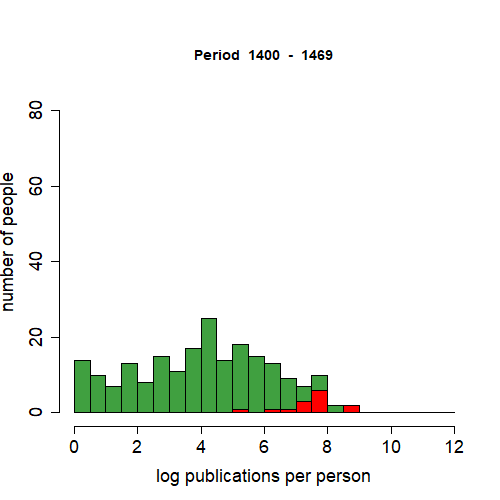
\includegraphics[width=.49\textwidth]{histo1Q.pdf}
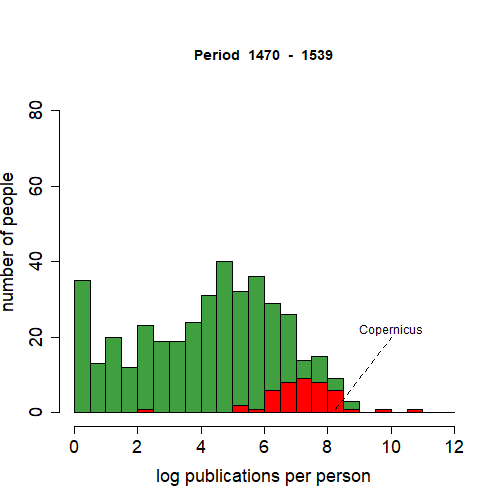
\includegraphics[width=.49\textwidth]{histo2Q.pdf}

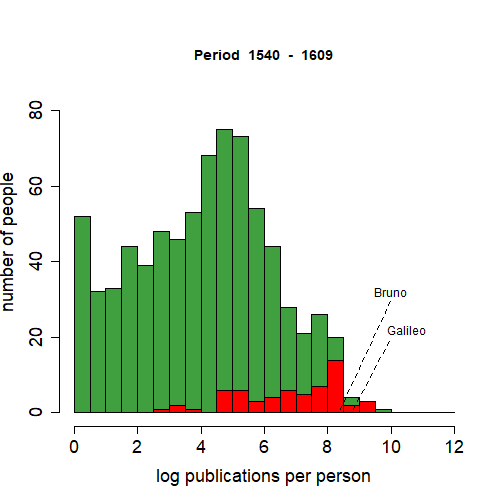
\includegraphics[width=.49\textwidth]{histo3Q.pdf}
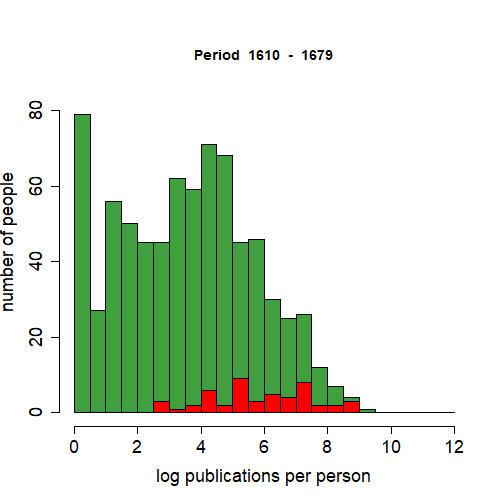
\includegraphics[width=.49\textwidth]{histo4Q.pdf}

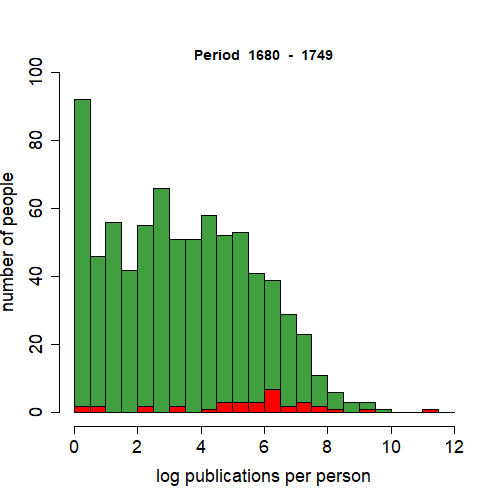
\includegraphics[width=.49\textwidth]{histo5Q.pdf}
\end{figure}

\begin{figure}[p]
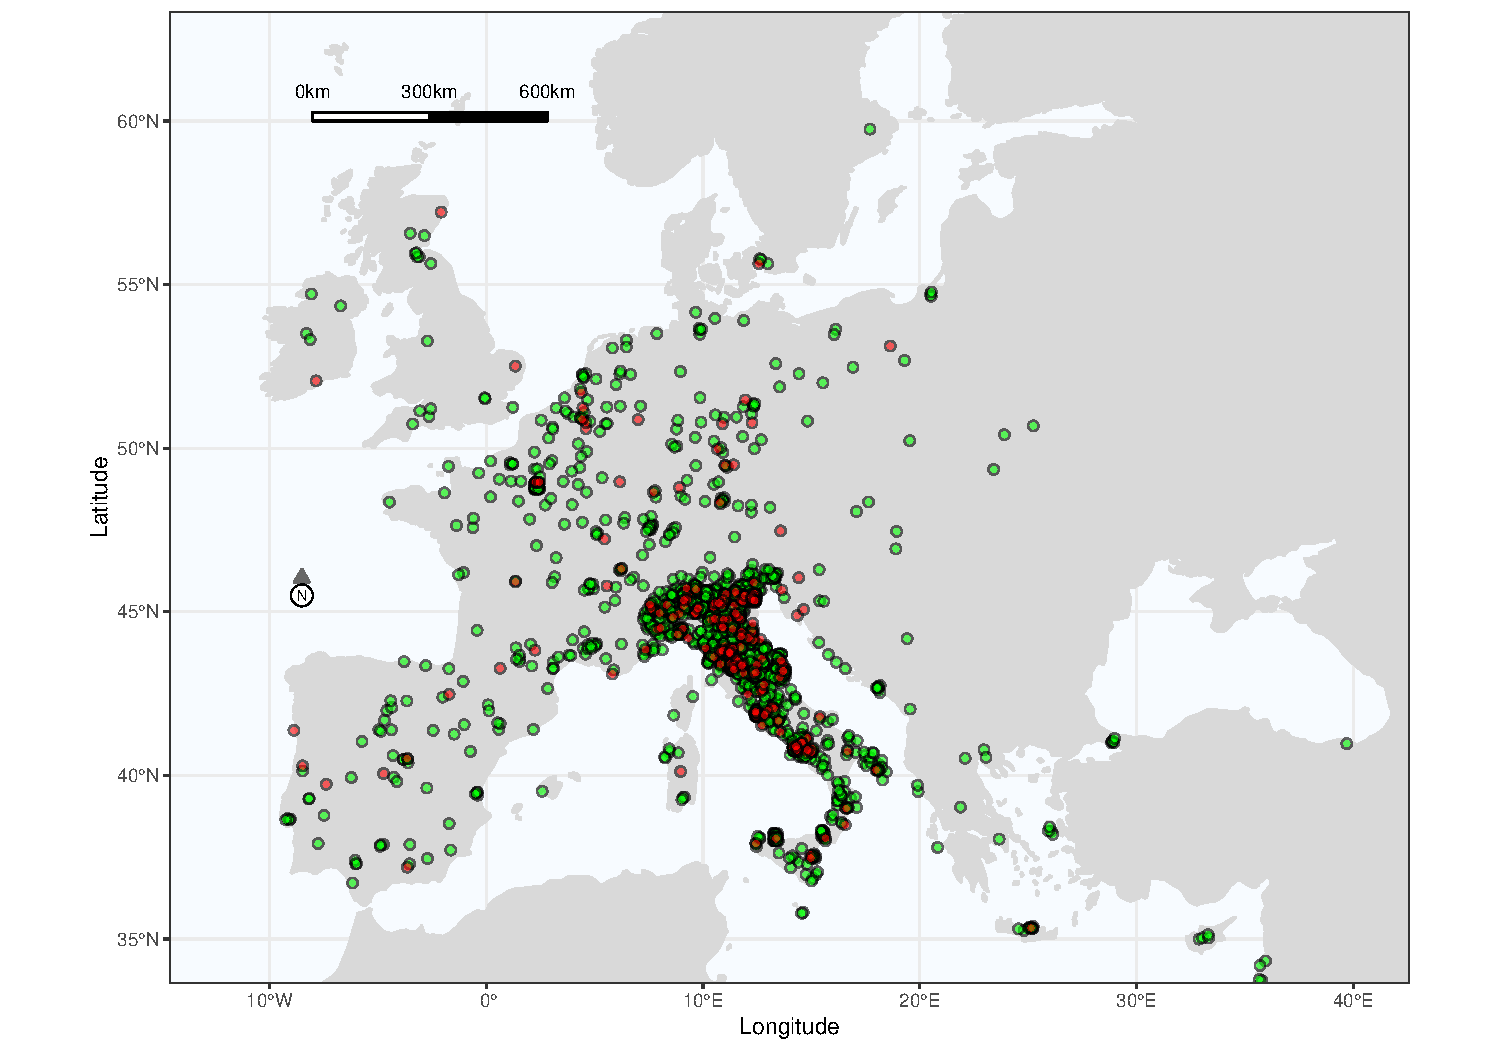
\includegraphics[width=.9\textwidth]{map-europe.pdf}
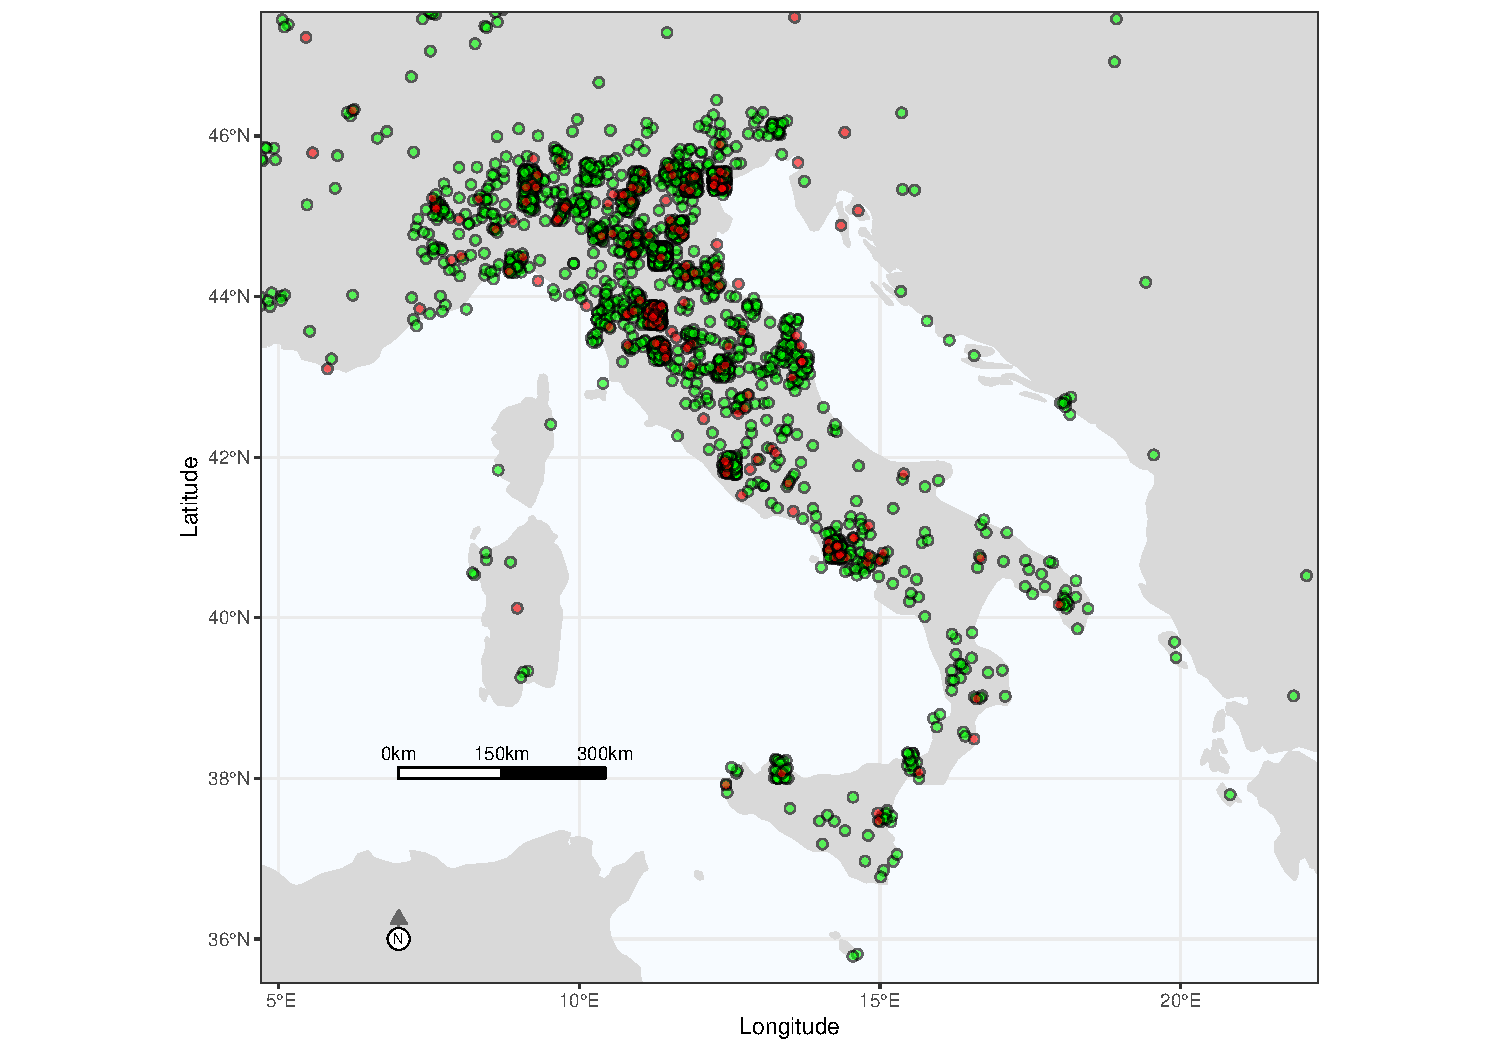
\includegraphics[width=.9\textwidth]{map-italy.pdf}
\end{figure}

\clearpage

\section{A Theory with Occupational Choice and Knowledge Diffusion}\label{section:theory}

In this section, we develop a theory of accumulation of knowledge and occupational choice. Authors, building on the knowledge left by the previous generation, write books that can be compliant to the ideology of the Roman Church or revolutionary (in the sense of the humanistic and scientific revolutions). Printers instead decide whether to be active in the revolutionary or compliant sector, and they make this choice according to the quality of the books of each type that they encounter. Therefore, if over time the revolutionary knowledge becomes better at a faster rate than the compliant one, the share of revolutionary books will also increase. The Roman Church dislikes revolutionary ideas and she might decide to censor them, which would decrease their share, but would also alter the accumulation of the total stock of knowledge in the economy.

\subsection{Knowledge Diffusion}

Time is discrete. At each date $t$ one generation is alive. Knowledge is embodied in books and is transmitted between the successive generations through them.\footnote{We do not underestimate the importance of tacit knowledge in the pre-industrial period -- see \citeN{de2017clans} -- but we are studying here how the church may affect knowledge exclusively through censoring books.} At the beginning of each period, the individuals first learn from $\mu$ books. $\mu$ is a parameter representing the number of books one can read during her live. Books include a more or less relevant content to produce goods and services. Irrelevance of a book read by person $i$ is denoted $h_{i}$. The productivity of someone using the knowledge in this book is
\begin{equation}\label{eq:qi}
q_i=h_i^{-\theta}, \;\;\; \theta\in(0,1).
\end{equation}

Books are of two types, which define different distributions from which their relevance is drawn.
 \textit{Compliant} books, indicated by the superscript $C$, embodies the type of knowledge is acquiescent with the ideology of the Roman Church,\footnote{Note that being compliant does not necessarily mean to produce using the official Roman Church doctrine as an input: this is true just for the production of religious books or religious services in general. Instead, it just mean that the knowledge should not contradict the Roman Church doctrine.} while \textit{revolutionary} books, denoted by the superscript $R$, indicates that the knowledge  is considered to be heretical by the Roman Church.

At the beginning of time $t$, the relevance of book $i$ of type $j$ follows an exponential distribution
\begin{equation}
h^j_i \sim \exp(k_{t-1}^j), \quad \text{with} \ j\in \{C,R\} \ \text{and} \ i\in \{1,..,N\}.
\end{equation}
whose scale parameter $k_{t-1}^j$ depends on the type of book. As
$$
\mbox{E}[h^j_i]=\frac{1}{k^j_{t-1}},
$$
$k^j_{t-1}$ measures the usefulness of knowledge in sector $j$.

Since the irrelevance of books is exponentially distributed and given \ref{eq:qi}, the distribution of book quality follows a Fréchet distribution with scale parameter $k^\theta$ and shape parameter $1/\theta$. This allows us to write the average book quality $\bar{q}^j$ by sector as:
\begin{equation}
E(q^j_i)=\int_0^\infty h^{-\theta}_i (k^j e^{-k^j h_i})dh_i=(k^j)^{\theta}\Gamma(1-\theta)\quad \text{with} \ j\in \{C,R\} \ \text{and} \ i\in \{1,..,N\},
\end{equation}
where $\Gamma(x)=\int_0^\infty s^{x-1} e^{-s}ds$ is the Euler gamma function.

The number of revolutionary books that each agent will read in $t$ depends on their availability in bookshops. The share of printers that produced revolutionary books in the previous generation is denoted by  $m_{t-1}$. Therefore, a individual will read $\lfloor \mu m_{t-1} \rfloor$ revolutionary books  and $\lfloor \mu (1-m_{t-1}) \rfloor$ compliant books, draw from their respective distribution. Each individual retains the best book coming from each one of the two distributions.
  Formally, the process of retaining the best books by sector is described as
\begin{align*}	
   \hat{h}^C_i&=\text{min}\{h^C_1,..,h^C_{\lfloor(1-m_{t-1}) \mu\rfloor}\},
 \\ \hat{h}^R_i&=\text{min}\{h^R_1,..,h^R_{\lfloor m_{t-1} \mu \rfloor}\}.
 \end{align*}
 For the sake of simplicity, from now on we will approximate $\lfloor(1-m_{t-1}) \mu\rfloor$ and $\lfloor m_{t-1} \mu \rfloor$ to respectively  $(1-m_{t-1}) \mu$ and $m_{t-1} \mu $, so that we will be able to proceed our analysis treating the number of books read as a continuous variable.

Given that the exponential distribution satisfies the minimum stability postulate according to which if $x$ and $y$ are mutually independent random variables, exponentially distributed with parameter $\lambda$, then $\min(x,y)$ is exponentially distributed with parameter $2\lambda$, we have:
\begin{align*}
\min\{h^C_1,..,h^C_{(1-m_{t-1}) \mu}\}& \sim \exp(k^C_{t-1} (1-m_{t-1}\mu) \mu),\;\;\;\mbox{ and }\\
\min\{h^R_1,..,h^R_{ m_{t-1} \mu }\}& \sim \exp(k^R_{t-1} m_{t-1} \mu).
 \end{align*}
We can now deduce that the distribution of actual relevance of the best book read by person $i$ follows
\begin{equation}
 \hat{h}^j_i \sim \exp(b_t^j), \quad \text{with} \ j\in \{C,R\},
\end{equation}
where $b_t^C$ and $b_t^R$ are defined as
 \begin{align*}
  b_{t}^C&=k_{t-1}^C (1-m_{t-1}) \mu, \\
  b_{t}^R&=k_{t-1}^R m_{t-1}  \mu.
 \end{align*}

Later in life, the generation $t$ writes new books,  combining their inherited knowledge with a new idea. This new idea is drawn from a distribution whose scale parameter depend on the average quality of the books they have read:
$$
h^j_N\sim  \exp(\nu b^j_t), \quad \text{with} \ j\in \{C,R\}.
$$
Taking the best of their acquired and new knowledge leads to a book with irrelevance distributed as:
$$
\tilde h^j=\min(h^j_N,\hat h^j) \sim  \exp((1+\nu) b^j_t).
$$
We can now summarize the dynamics of the two types of knowledge by the dynamics of the scale of their distribution:
 \begin{align}
  k_{t}^C&=(1+\nu) k_{t-1}^C (1-m_{t-1}) \mu,\label{eq:kCtime} \\
  k_{t}^R&=(1+\nu) k_{t-1}^R m_{t-1} \label{eq:kRtime} \mu.
 \end{align}


 \subsection{Occupational Choice}

 To finish the description of the dynamics we need to define now how the  share of  printers  producing revolutionary books evolve over time.
We suppose that printers meet authors randomly, but have to decide where to be active in the compliant sector or in the revolutionary sector at the beginning of their activity. Once they have chosen a sector\footnote{Assuming that printers has to choose a sector is consistent with \citeN{dittmar2015}. In Germany, the official city printers were not advocates of the Reformation because they “did not want to endanger official work orders or antagonize city governments". Moreover, according to \cite{grendler1975}, printers in Venice faced the risk of having their bookshops in Rome sized by the Vatican if they printed revolutionary content, which implies that they had to choose a sector.}, they would print any author they meet randomly. They will thus determine their sector of activity based on the first author they meet. This author has written books of relevance $\tilde{h}^C$ and $\hat{h}^R $. Printers decide their sector taking into account both the relative relevance of the two books and the fact that customers of the bookshop might value differently two books with the same quality that belong to two different sectors. This might happen because of consumer preferences or for how book quality translates into consumption goods\footnote{Books can be used to produce consumption goods and books belonging to different sectors can have different productivity in this respect. For example the production of consumption goods through books can be represented as $c=\alpha\sum^{N_R} q_i^R+\sum^{N_C} q_i^C$, where $\alpha$ would be the relative productivity of revolutionary books quality, while $N_R$ and $N_C$ are respectively the number of revolutionary and compliant books owed by the customer.}. We summarize these two effects assuming that the relative price\footnote{The price can also reflect the risk of being caught selling forbidden books.} at which revolutionary books can be sold is represented by $p$.  The probability that the revolutionary book is best is:
\begin{equation}
\text{Prob}\{q^C<p q^R\}=\text{Prob}\{\tilde{h}^C>p^{-1/\theta}\tilde{h}^R\}=\frac{b^R_t}{b^R_t+b^C_t p^{-1/\theta}}=m_t.
\end{equation}
Using the law of large numbers, this probability also defines  the share of printers active in the  revolutionary sector $m_t$. From now on we will refer to $\hat{p}$ as $\hat{p}=p^{-1/\theta}$.

The dynamics of knowledge quality (\ref{eq:kCtime}) and (\ref{eq:kRtime}),  together with the occupation choice
\begin{equation}\label{eq:sharer}
m_t=\frac{k^R_t}{k^R_t+\hat{p}k^C_t}
\end{equation}
and initial conditions $k_{-1}^C$ and $k_{-1}^R$, determine the equilibrium path $\{ m_t,  k_{t}^C,  k_{t}^R\}_{t\geq 0}$.

 Assuming that printers determine their sector of activity based on the first author they meet is equivalent to say that they choose their sector according to the best available book in the bookshop. It is rational for printers to choose their sector as we described and not comparing the average qualities by sector if customers, which are the target of printers, purchase the best available book in the bookshop. This interpretation also requires printers to be aware that $\text{Prob}\{\tilde{h}^C>\hat{p}\tilde{h}^R\}=\text{Prob}\{\hat{h}^C>\hat{p}\hat{h}^R\}$: this is important because they need to know that the probability that the best book in the bookshop is revolutionary is the same that a revolutionary book is the best among new titles.

\subsection{Censorship}\label{subsection:censor}

So far the Church did not play any role in the model. As we discussed in the introduction, there is historical evidence that the Roman Church tried to limit the spread of revolutionary books issuing the \textit{Index Librorum Prohibitorum}. We model this behavior of the Church assuming that she can interfere  with the process of occupational choice imposing a rate of censorship on revolutionary books. More precisely, she can limit the number of revolutionary titles that an author can read, making unavailable a fraction $\beta$ of the volumes that she would have read without censorship. Formally, the process of censorship limits the number of revolutionary books that individuals encounter during their life to $\mu m (1-\beta)$ and therefore alters the process of accumulation of revolutionary knowledge, which now follows
\begin{equation}\label{eq:censorhip}
k_{t}^R=(1+\nu)(1-\beta)k_{t-1}^R m_{t-1} \mu, \quad\text{with} \ \beta\in[0,1].
\end{equation}
Note that in this way they Church can directly decrease share of revolutionary books $m$ and will also make less likely that revolutionary works will be written in the future, since the process of accumulation of revolutionary knowledge slows down.

History tell us that book's censorship was not the only way the Church used to limit the spread of revolutionary books: in fact, in the second half of the $16^{\text{th}}$ century, the Roman Church developed a system of tribunals, called \textit{Roman Inquisition}, aimed at persecuting both authors and printers accused of heresy. This institution affected the work of scientists and thinkers: a notable example is the process to Galileo Galilei, who was tried by the Inquisition in 1633. The inquisition matters for our analysis because it can slow down the accumulation of revolutionary knowledge through self-censorship: even if one author writes a high quality revolutionary book, she still might prefer not to hand it in it to the printer for the fear of being processed by the Inquisition. Similarly, even if the best books are revolutionary, the printer might still prefer to be compliant for the same reason. This mechanism can be easily incorporated in our framework assuming that the Inquisition makes publishing and writing revolutionary books less desirable, which individuals take into account discounting $q^R$ by a factor $\gamma\in[0,1]$. We can also interpret $\gamma$ as the probability that authors decides not to write revolutionary books or that printers do not publish them for the fear of receiving a punishment. Under this new mechanism, probabilities that the revolutionary sector is chosen by a printer is:
\begin{equation}\label{eq:censorhip2}
\text{Prob}\{q^C<\gamma p q^R\}=\text{Prob}\{\tilde{h}^C>(\gamma p)^{-1/\theta}\tilde{h}^R\}=m_t.
\end{equation}
\subsection{The Dynamics under an Exogenous Church's Behavior}
So far we mentioned that the Church can limit the share of revolutionary books through censorship, but we did not mention how the Church is choosing $\beta$. Clearly, the choice of  $\beta$ over time will depend both on the behavior of agents, which is described in the previous section, and on the objective of the Roman Church. One one hand, it is clear that the Church wanted to have the smallest possible number of heretical books circulating in order to maintain her power, but on the other hand we do not know what was preventing her to impose the highest level of censorship in any period. It seems that the Church was trading-off censorship with something else, which could be time spent in other activities of her interest or the fact that a too harsh censorship would have created an economic damage to the Church itself,\footnote{As an example, we can think that if the censorship is too harsh, the Roman Church might lose in terms of competition with the Protestant Church, since devotees dislike a too harsh censorship.} or something else.

Here we treat $\beta$ as is it was exogenous, and we study the dynamics under this assumption. We start defining $z=k^R/k^C$: note that the share or revolutionary ideas $m$ can assume one and only one value given $z$, which means that once we know the dynamics of one of the two variables, we will also know the dynamics of the other. From equation (\ref{eq:sharer}) we get
\begin{equation}
m_t=\frac{z_t}{\hat{p}+z_t}\label{eq:sharer2}.
\end{equation}
 We decided to make $m_t$ rather than $z_t$ our main variable for describing the model dynamics because its domain is a bounded set.
 The dynamics of $m$ are defined formally below.
\begin{definition}\label{definition:equilibrium}
	Given $\beta$, an equilibrium path is a sequence $\{m_t\}_{t\geq0}$, describing the share of revolutionary books over time. It is such that:
	\begin{itemize}
	\item Each author of each generation write books whose quality and type is defined by the current state of knowledge.
	\item Each printer of each generation chooses her sector according to the most productive book presented by the first randomly met author.
	\item Each printer of each generation, once she chose her sector, prints all the authors she meets randomly.
	\item The probability of being exposed to revolutionary book in $t+1$ depends on the share of revolutionary titles written in $t$.
	\end{itemize}
\end{definition}
The equilibrium described in definition \ref{definition:equilibrium} depends on the whole theory that we described in the previous subsection, but we are able to summarize in a single equation the law that governs the dynamics of $m$.
Dividing Equation~(\ref{eq:kRtime}) by (\ref{eq:kCtime}) side by side, and substituting the resulting $z_{t+1}$ in (\ref{eq:sharer2}) at time $t+1$, we get the equation that governs the equilibrium dynamics of $m$:
\begin{equation}
m_{t+1}=\frac{(1-\beta) m_t^2}{1-m_t ((\beta -2) m_t+2)}=f(m_t)\label{eq:lawm}.
\end{equation}
Equation~(\ref{eq:lawm}) together with an initial condition $m_0$, allow us to determine the equilibrium path $\{m_t\}_{t\geq0}$. Using the variable $z_t$, Equation~(\ref{eq:lawm}) can be rewritten as
$$
z_{t+1} = \frac{1-\beta}{\hat{p}} (z_t)^2.
$$
This recurrence equation admits an explicit solution:
\begin{equation}
z_t=\frac{\hat{p}}{1-\beta}{\left(\frac{z_0 (1-\beta)}{\hat{p}}\right)^2}^t.
\end{equation}

The equilibrium path $\{m_t\}_{t\geq0}$ thus satisfies:

\begin{proposition}
	Given the initial condition $m_0$, we have
	\begin{itemize}
    \item[i)]$\lim_{t\to\infty}m_t=0$ if $m_0<1/(2-\beta)$,
    \item[ii)] $\lim_{t\to\infty}m_t=1$ if $m_0>1/(2-\beta)$,
     \item[iii)]$\lim_{t\to\infty}m_t=m_0$ if $m_0=1/(2-\beta)$.
	\end{itemize}
    More in particular, with full censorship, or with $\beta=1$, the share of revolutionary ideas converges immediately to 0, unless $m_0=1$: in this case we will have $m_t=1 \ \forall \ t\geq0$.
	 \label{proposition:dynex}
\end{proposition}

\begin{proof}
Given the change of variable, $m_0<1/(2-\beta) \Leftrightarrow z_0<\hat{p}/(1-\beta)$. In that case, $lim z_t =0$ and $\lim m_t=0$. We also have that
$m_0>1/(2-\beta) \Leftrightarrow z_0>\hat{p}/(1-\beta)$. In that case, $lim z_t =+\infty$ and $\lim m_t=1$. Similarly, when $z_0=\hat{p}/(1-\beta$), $z_t=\hat{p}/(1-\beta)$ for all $t$, and $m_t=1/(2-\beta)$ for all $t$.
\end{proof}

\subsection{The Dynamics under a Rule of Thumb Church's Behavior}
In the previous subsection we described the dynamics under a constant rate of censorship $\beta_t$. We also observed that the Church wanted to have the smallest possible level of revolutionary books, but at the same time imposing censorship was costly to her for many possible different reasons. Here we do not want to take a stand on the global objective of the Church, but we rather assume that she will choose the lowest rate of censorship that will allow the converge to a world with no revolutionary ideas. This is equivalent to assume that the Church has lexicographic preferences, caring firstly to have $\lim_{t\to\infty}m_t=0$, and secondly to minimize $\beta_t$. Given our assumptions, we are able to describe the dynamics of the share of revolutionary ideas in Proposition \ref{proposition:rthumb}.
\begin{proposition}
	For a given share of revolutionary ideas $m_t \in [0,1)$, the Church will choose a level of censorship $\beta_t$ such that $\beta_t=\max\{2-1/m_t+\epsilon,0\}$, where $\epsilon$ is arbitrarily small. If $m_t=1$, it does not exist a rate of censorship $\beta_t \in [0,1]$ such that $\lim_{t\to\infty}m_t=0$.
	\label{proposition:rthumb}
\end{proposition}
\begin{proof}
For the case $m_t=1$, the result follows directly from Proposition \ref{proposition:dynex}. For the case $m_t \in [0,1)$, notice that \ref{proposition:dynex} states that $\lim_{t\to\infty}m_t=0$ when $m_t<1/(2-\beta_t)$, from which trivially follows  $\beta_t=\max\{2-1/m_t+\epsilon,0\}$.
\end{proof}
\newline\\
It is trivial to note that for any initial $m_0 \in [0,1)$, we will have $\lim_{t\to\infty}m_t=0$, even though the convergence will be slow due to the fact that in any period $m_t$ would be set very close to the unstable steady state $1/(2-\beta_t)$. It is worth noting that Proposition \ref{proposition:rthumb} implies that the Church will impose no Censorship if $m_t<1/2$.
\subsection{The Dynamics under an Optimizing Church's Behavior}
In the previous subsection we described the Church's behavior and the evolution of heretical books over time using a parsimonious model. On one hand, this approach had the strength of making just minimal assumptions concerning the Church's objectives, but, on the other hand, it lead to two main shortcomings. Firstly, it is actually stringent in defining the way the Church trades off the prevalence of revolutionary books and censorship. Secondly, it leaves unexplained why censorship rapidly moved from 0 to a considerable amount\footnote{It is unlikely that this is due to a sudden blow of revolutionary ideas. In fact, some books were not subject to censorship at the time they were published, but were suddenly forbidden at a certain point later on in history. A notable example is Dante's \textit{De Monarchia}, which was first published in 1312, but it was forbidden in 1585 only.} in a few decades. Here we propose a model that is able to address this additional fact, other than explaining the two features of authors censorship that we illustrated in Section \ref{section:twof}. Our idea is that setting up an apparatus able to create a list of forbidden books and enforce its application represented a large fixed cost to bear for the Church. Therefore, we assume that the Church cannot enforce any censorship before having paid a fixed cost $\psi$, that allows her to impose a rate of censorship up to $\overline{\beta}$. The Church care about the share of compliant books in the economy: her utility function is given by $u()$, which is differentiable, bounded and strictly increasing in $1-m_t$, while $\delta<1$ is the discount factor. We can now define recursively the value function of Church if she still did not established a censorship structure yet:
\begin{equation*}	
	V(m_{t-1})=\max[V^N(m_{t-1}),V^C(m_{t-1})-\psi],
\end{equation*}
where $V^{N}$ is the value of not imposing censorship and equals
\begin{align*}
V^{N}(m_{t-1})&=u(1-m_{t})+\delta V(m_{t})	\\
	 \text{s.t.}\quad m_{t}&=f(m_{t-1},0)=\frac{ m_{t-1}^2}{1-m_{t-1} (-2 m_{t-1}+2)},
\end{align*}
while $V^{C}$ is the value of having a censorship apparatus set up and equals
\begin{align*}
V^{C}(m_{t-1})&=\max_{0\leq\beta_t\leq\overline{\beta}}u(1-m_{t-1})+\delta V^C(m_{t}),	\\
	 \text{s.t.}\quad m_{t}&=f(m_{t-1},\beta_t)=\frac{(1-\beta) m_{t-1}^2}{1-m_{t-1} ((\beta -2) m_{t-1}+2)}.
\end{align*}
Note that we could write this last value function like that since $V^N(m_{t-1})$ equals $V^C(m_{t-1})$ if $\beta=0$ is chosen. Moreover, it is straightforward to see that, once $\psi$ has been paid, the Church will always set $\beta_t$ to its maximum level\footnote{This holds because $\partial f(m_{t-1},\beta_t)/\partial\beta_t\leq 0$ and $\partial u(1-m_t)/\partial m_t<0$, which imply $\partial V^C(m_t)/\partial \beta_t\geq 0$.}. In this model the Church has to choose between paying a fixed cost today for having the possibility to enjoy a lower share of revolutionary books in the future and postponing such payment, which would make censorship less costly because of discounting, but it would also imply a higher share of revolutionary books in the future. This trade off implies that the Church would be more prone to implement censorship immediately when the fixed cost $\psi$ is low and when the effectiveness of censorship $\overline{\beta}$ is high. Moreover, she is less inclined to start censoring immediately if she is more impatient: when $\delta=0$, the Church cares only about what happens in 0, and therefore she will never pay a cost $\psi$ that affects only the future share of revolutionary books.
Other than parameters, the Church's decision about whether and when to start censoring crucially depends on the initial level of revolutionary books $m_{-1}$, because it influences the dynamics of $m$ and hence also the differences in the dynamics under censorship and without it. To gain intuition about why the initial condition matters, consider the extreme cases $m_{-1}=0$ and $m_{-1}=1$: Proposition \ref{proposition:dynex} states that in both situations $m$ will stay constant over time, regardless of the value of $\overline{\beta}$, which clearly makes censorship useless.
While we have already showed qualitatively how parameters and initial conditions are expected to influence the Church's decision, Proposition \ref{proposition:tooLate} allow us to better understand when it is not optimal for the Church to censor:
\begin{proposition}
\label{proposition:tooLate}
If $\psi>0$, $\exists\;\tilde{m}>0,1>\breve{m}>0$ such that
\begin{itemize}
\item[i)] If $m<\min(1/2,\tilde{m})$ then $\beta_t=0\;\forall t\geq0$ (No need to censor),
\item[ii)] If $m>\max(1/2,\breve{m})$ then $\beta_t=0\;\forall t\geq0$ (Too late to censor).
\end{itemize}
\end{proposition}
\begin{proof}
Note that $u(0)/(1-\delta)=V^N(0)>V^C(0)-\psi=u(0)/(1-\delta)-\psi$ and $u(1)/(1-\delta)=V^N(1)>V^C(1)-\psi=u(1)/(1-\delta)-\psi$. Now, note that $V^M(m)$ and $V^C(m)$ are continuous functions in $m_{t-1}\in[0,1]$: see \citeN{norets2010} for a formal proof of continuity of discrete choice dynamic value functions under a set of assumption that are satisfied in our case. Then, it follows that there exists $\tilde{m}$ and $\breve{m}$, respectively in a neighborhood of 0 and 1, such that $\forall m\in[0,\tilde{m}]$ and also $\forall m\in[\breve{m},1]$, it holds $V^N(m)>V^C(m)-\psi$. Proposition \ref{proposition:dynex} completes the proof.
\end{proof}

Proposition \ref{proposition:tooLate} makes the point that for some $m_{t-1}$ it can be optimal for the Church to never impose Censorship, and this can be due to opposite reasons. In fact, for a low enough $m_{t-1}$ the Church knows that revolutionary ideas would naturally disappear and therefore there is no need to censor: if the initial $m_{t-1}$ is close enough to the compliant steady state, the gain of forbidding would be very low because there is no room for changing much future $m_{t-1}$, and therefore censorship will be never imposed. Symmetrically, when $m_{t-1}$ is high enough, the Church knows that even imposing Censorship she would converge  fast to the revolutionary steady state: in this case it is too late to censor.
So far we did not discuss for for which parameter values and states the Church is willing to impose censorship: while it is not possible to fully characterize these conditions, Proposition \ref{proposition:window} tell us that under some conditions on the parameters we are able to say that for some $m_{t-1}$ the Church will start censoring.
\begin{proposition}
\label{proposition:window}
$\exists\;\overline{\psi}$ such that $\forall$ $\psi<\overline{\psi},\;\;\exists \;\overline{m},\hat{m}$ such that for $\hat{m}>m_{-1}>\overline{m}$ it holds $\beta_0=\overline{\beta}$ (Window of censorship).
\end{proposition}
\begin{proof}
We take $\overline{\psi}$ such that for some $m^*$ we have $V^C(m^*)-\overline{\psi}>V^N(m^*)$, then $\forall \;\psi<\overline{\psi}$ it holds $V^C(m^*)-\psi>V^N(m^*)$. Now define $\mathcal{D}(m)=V^C(m)-\psi-V^N(m)$: since this function is continuous, for an arbitrarily small $\epsilon$ we have that $\mathcal{D}(m^*-\epsilon)>0$ and $\mathcal{D}(m^*+\epsilon)>0$. Using again continuity we can claim that $\mathcal{D}(m)>0\;\forall\;m\in[m^*-\epsilon,m^*+\epsilon]$, which implies that the church will immediately impose censorship if $m_{-1}$ belongs to this set.
\end{proof}

Proposition \ref{proposition:window} tell us that the areas under which the church is willing to censor are not isolated points, but instead form \textit{windows} that do not include the boundaries\footnote{Unless $\psi$=0.} of the domain of $m$. This result is intuitive if we think that two conditions should hold to make the Church willing to censor. First, censorship should be able to alter significantly the time path of revolutionary books, where the extreme case would be to change the steady state to which $m_t$ converges from revolutionary to compliant. Secondly, the Church should lose the opportunity to change dramatically the equilibrium path through censorship if she waits one additional period for doing so. Censorship decisions are not taken in isolated points because contiguous points have a very similar value of postponing censorship and of altering the dynamics of $m$ through forbidding, which vanishes when $m$ gets closer to the boundaries.

Notice that we did not characterize the equilibrium time path $\{m_t\}_{t\geq0}$ for different values of the parameters: the reason is that censorship \textit{windows} can be placed anywhere in $[0,1]$ unless some strict assumptions are made. Moreover, the discrete nature of our problem can create situations under which very close initial conditions deliver very difficult equilibrium paths, because the censorship windows are ``jumped". While we cannot fully characterize the equilibrium time path, the model leaves open the possibility that revolutionary ideas were growing or declining before censorship was first implemented. One test of the model would be to find after the calibration that revolutionary ideas were actually growing before the censorship, which is accordance with the historical fact that the Protestant reformation started before the first issue of the \textit{Index Librorum Prohibitorum}. One last thing is worth noting: the parameters $\delta$ and $\psi$ matter for the time $t$ at which the Church decides to set up censorship, but once $t$ is decided, the dynamics of $m_t$ evolve independently of them. Therefore, in Section \ref{section:identification}, we will provide a combination of $\delta$ and $\psi$ consistent with the introduction of censorship at a certain point in time, but we will not be able to identify them.

\subsection{Discussion of Model Assumptions}
Our model of censorship introduction under an optimizing Church's behavior relies on a set of assumptions that allowed us to make it tractable. In this subsection we discuss such assumptions and we compare them with some alternative modeling choices that we could have taken.

A point that is worth discussing is that in our model the Church will always set censorship to its maximal level $\overline{\beta}$ once $\psi$ has been paid. Alternatively, we could have assumed that the Church cared about not hampering too much the accumulation of knowledge, which in turn would have given to her the incentive to choose an intermediate value of $\beta_t$ in some cases. This alternative model could explain the empirically observed decline in $m_t \beta_t$ through a decrease in the rate of censorship rather than through a drop in the prevalence of revolutionary ideas. Nevertheless, historians did not report a clear decrease in the strictness of censorship over time. Some books appeared in the index under the heading \textit{donec corrigatur}, which means that the book is forbidden until a correction of the book appear, but the Vatican rarely\footnote{One of the few cases is represented by the \textit{Index expurgatorius}, which contained 50 titles only and was suspended by the Inquisition in 1612, seven years after its presentation (\citeNP{wolf2006}, 34).} issued such corrections, meaning that the diffusion of knowledge was not a priority. Moreover, while the disagreement within the Church affected her policy, sometimes causing revisions of the most intransigent positions, the censorship trend displayed increasing rigidity (\citeNP{balsamo2001}, 13).

A different modeling choice that we could have taken is to assume that there is no fixed cost $\psi$ to be paid, but rather a cost which depends on how large is the $\beta_t$ that has been set. A model based on this alternative assumption would be hard to reconcile with the data, because it would not be able to reproduce a "jump" in the number of books censored like the one we could observe in the data. In fact, this alternative model would rather predict a gradual increase or decrease in the share of forbidden books, and it would also generate a faster reaction to the diffusion of Protestantism than the one observed in the data.

Another possible modeling choice would have been to assume that the Church is not limited to censor up to a \textit{fraction} of all the existing revolutionary ideas, but rather to censor up to a certain number of books [For David: if you think that this paragraph is not convincing, I will solve and estimated this variant of the model]. Here we claim that this assumption is not better than ours at describing how censorship was actually enforced in early modern Italy. \citeN{prosperi2010} reports that the \textit{Congregation of the Index}, which was the organization responsible for the introduction of new titles into the index, was formed of eight cardinals only in 1587, while previously it had been five. Moreover, \citeN{wolf2006} observes that between 1571 and 1596, the number of yearly meetings of the congregation oscillated between 0 and  and 34. These pieces of evidence suggest that the Church was not constrained by total number of books she could possibly analyze, because she could have easily increased them through an rise in the number of cardinals in the congregation or multiplication of the number of yearly meetings. Instead, what was preventing the Church from censoring all revolutionary books was the existence of frictions in the rate of arrival of new books to check. In fact, it has been pointed out (\citeN{wolf2006} and \citeN{prosperi2010}) that the censoring \textit{iter} most of the times started by an external denounce\footnote{By external denounce we mean that the process was not initiated by the congregation itself. \citeN{wolf2006} enumerate members of the clerics, aristocrats and bourgeoisie as the categories of people that were bringing a book to Rome for denouncing it.}. If arrival rate of new books was low enough, then the Church did not have the opportunity to censor all revolutionary books, but just a fraction of them.

One additional assumption we made is that the Roman Inquisition was able to enforce the application of the index outside the Vatican and over time.
The main weapon of the Church for enforcing the application of the index was a dense peripheral organization of censorship, which was constituted by 41 inquisitorial tribunals, mostly distributed in northern Italy, and by bishops in the center-south\footnote{In the south and in the highlands the inquisition was carried on by the Spanish, with exception of Naples, where the archbishop was responsible for censorship (\citeNP{prosperi2010}).} (\citeNP{balsamo2001}). Moreover, the Church had an additional economic weapon for enforcing censorship which is directly linked to printers. \citeN{grendler1975} studies the case of Venice and claims that the Church originally enforced compliance threatening printers to seize their stores within the papal state. These menaces would work as long as the volume of revolutionary ideas stays low, otherwise printers would prefer to start printing the demanded revolutionary books, even at the cost of losing their businesses in Rome. Concerning the span of time during which censorship was actually implemented, \citeN{prosperi2010} claim that it continued throughout the XVIII century, even thought it became harder for the Church at the end of this period to enforce the application of the index. In fact, under the papacy of Pope Benedict XIV, which started in 1740, some inquisitorial tribunals were closed. Therefore, we can claim that our assumption about censorship enforcement is valid until the first half of the XVIII century.

\section{Identification of the Parameters}\label{section:identification}

Here, we estimated the parameters of the model if occupational choice and optimizing Church's behavior described in Section \ref{section:theory}, using the data described in Section \ref{section:data}. Estimating the model from the data will allow us to compute the effect of censorship on knowledge production through running a counterfactual experiment where the censorship rate has been set to zero.

First, for taking our model to the data we need to decide what is the empirical counterpart to the periods in the model. We want our division of time to respect four conditions: first, we want each period to correspond to an equal number of years. Second, we want to stop in 1750, both because the Church might have lost her capacity to censor for reason external to our model and because our data source about Italian Academies stops in 1700. Third, we want that a year close to 1544, which corresponds to the first Index of Paris, to be the threshold of the separating the last period without censorship and the first period with it. Finally, we don't want each period to be too short, otherwise the standard errors of our variables of interest would be too large due to the small number of authors in each period. These considerations led us to create 5 periods: 1400-1470, 1470-1540, 1540-1610, 1610-1680 and 1680-1750. We have a total of 8 parameters\footnote{We are actually left with 9 parameters, but we cannot distinguish between the number books read by authors, $\mu$, and the parameter governing the relative productivity of new ideas, $\nu$. In fact, they both matter for growth in books quality only, which is governed by $(1+\nu)\mu$, which is the combination of parameters that we will estimate.} to be pinned down and Table~\ref{table:param} summarizes our strategy: we will first calibrate two of them, while the rest will be estimated. We set the discount factor $\delta$ such that it matches a yearly discount factor of $0.99$ for a given period length $T$: $\delta=0.99^{T}$. The other calibrated parameter is $\psi$, which is taken such that, given the time path implied by the other 7 parameters under the assumption that censorship kicks in  $t=3$, is able to rationalize the timing at which censorship starts. This parameter is not identified: there exists a range of values that are able to rationalize the timing of a start of  censorship.
We are left with 6 parameters that we will estimate using the simulated method of moments. The moments use for the estimation are the median and the $75^{th}$ percentile of the overall and revolutionary distribution of quality, as well as the share of censored ideas. We target the median instead of the mean because it is less sensitive to outliers, while we target the $75^{th}$ percentile of the quality distribution to identify $\theta$, which governs the shape of the Fréchet distribution. It is worth nothing that we target censored ideas in $t=1$: we assume that the Church in $t$ cannot only censor books in $t-1$, but she can target all the past volumes. Even if censoring books older than $t-1$ do not influence future dynamics\footnote{Since the marginal cost of censorship is zero in the model and variables in $t$ are only affected by variables in $t-1$, all the dynamics described in Section \ref{section:theory} remains identical.}, we made this assumption to avoid throwing away informative data. In fact, under the assumption of a constant rate of censorship, $m_2\overline{\beta}>m_1\overline{\beta}$ implies that the share of revolutionary ideas is growing. In total we have 25 target moments. The parameters are taken such that the distance between the empirical and simulated moments is minimized, formally
\begin{equation}
\hat{q}=\arg\min_{q} (\mathbf{m}-\mathbf{m}_q)'\mathbf{W}(\mathbf{m}-\mathbf{m}_q),
\end{equation}
where $q$ is a vector of parameters, $\mathbf{m}$ is the vector of data moments and  $\mathbf{m}_q$ is the vector of moments obtained simulating the model with parameters $q$. $\mathbf{W}$ is a diagonal matrix with $1/\mathbf{m}^2$ as elements. Since the objective function might not be well-behaved, we minimize the objective function using the genetic algorithm package in R, developed by \citeNP{scrucca2013}, which allows for global optimization.
In order to support the precision of our estimates we compute bootstrapped standard errors of the parameters, drawing 100 new samples with replacement from the original data. The fact that standard errors, reported in Table~\ref{table:param}, are relatively small, suggests that the parameters of the model are well identified.
The model fit is reported in Figure \ref{fig:fit}. The simulated variables rarely lies outside the $95\%$ confidence interval\footnote{The confidence intervals are computed drawing 1000 random new samples with replacement and then using the $2.5^{th}$ and $97.5^{th}$ percentile from the distribution of the variable that interests us.} of the data moments: an exception is the missed increase and drop in $m_t \beta_t$ in the first two periods. While the fit of the model is good, nothing prevents that there exist another model with a fit that as good as ours. To further support that we are considering the true underlying mechanisms that are governing the dynamics of knowledge, we test the ability of the estimated model to reproduce data that was not used as a target. In Figure \ref{fig:over} we check the ability of the model to reproduce the median and the $75^{th}$ percentile of the distribution of non censored books. While we capture the drop in quality over time,  the level of book quality is slightly higher for the $75^{th}$ percentile: this is probably due to the fact that the logarithm of publications is not distributed like a Fréchet like in the model.


%%%%TABLE PARAMETERS%%%%%
\begin{table}[H]
  \centering % used for centering table
  \begin{tabular}{@{} l c c c @{}}  
  \hline\hline %inserts double horizontal lines
  \ External Parameters &  & Value & Target  \\ [0.05ex] % inserts table
    %heading
  \hline % inserts single horizontal line
  \rule{0pt}{2.5ex}
  Productivity of books  & $\theta$   & 0.18 & Variance of $q^R_1$  \\[0.15ex]
  Mean quality in 1  & $\overline{q}_1$   & 5.36 & First period quality  \\[0.15ex]
  Mean rev. quality in 1  & $\overline{q}^R_1$   & 7.67 & First period quality \\[0.15ex]
  \hline \hline
  \ Estimated Parameters &  & Value &  \\ [0.05ex] % inserts table
  \hline
  \ \%censored revolutionary books  & $\overline{\beta}$   & 0.15 & MSM  \\[0.15ex]
  TFP  & $(1+\nu)\mu$   & 1.66 & MSM  \\[0.15ex]
  Price of compliant books   & $p$   & 178.37 & MSM  \\[0.15ex]
  \hline
  \end{tabular}
  \end{table}



\section{The Role of Censorship for Knowledge Formation}
The question that we are asking in this paper is whether Catholic's church censorship was key in altering the path of knowledge accumulation in Italy. The fact of having estimated a structural model of occupational choice under an optimizing church's behavior, allow us to perform a counterfactual experiment where the Church did not set up a censorship apparatus, or equivalently $\overline{\beta}=0$. Figure \ref{fig:exp} illustrates the outcomes of this experiment. Without censorship, the share or revolutionary ideas $m_t$ would have had continued increasing over time, and both the overall and revolutionary books quality would be have been higher.  Only the quality of compliant books shows a slight decrease under the no censorship scenario, because the stock of knowledge used for producing compliant books is relatively lower. Note that the overall loss in knowledge quality due to censorship, which amounts to $23.6\%$ in the period 1680-1750, is both driven by the lower quality of revolutionary ideas and by the drop in $m_t$, because in all scenarios  revolutionary books quality is much higher that the compliant ones. More in particular, if $m_t$ in the baseline stayed the same as in the baseline, the drop would have been of $10.5\%$, suggesting that around half of the effect is driven by the change in quality within sectors, while the the rest is due to the switch from the revolutionary to the compliant sector. Note that these estimates are valid under the assumption that self-censorship did not play a role. In appendix \ref{appendix:b} we tackle this problem, estimating the variant of our model with self-censorship, as described in Subsection \ref{subsection:censor}. The results show that the role of self-censorship was minor.
\begin{figure}[htbp]
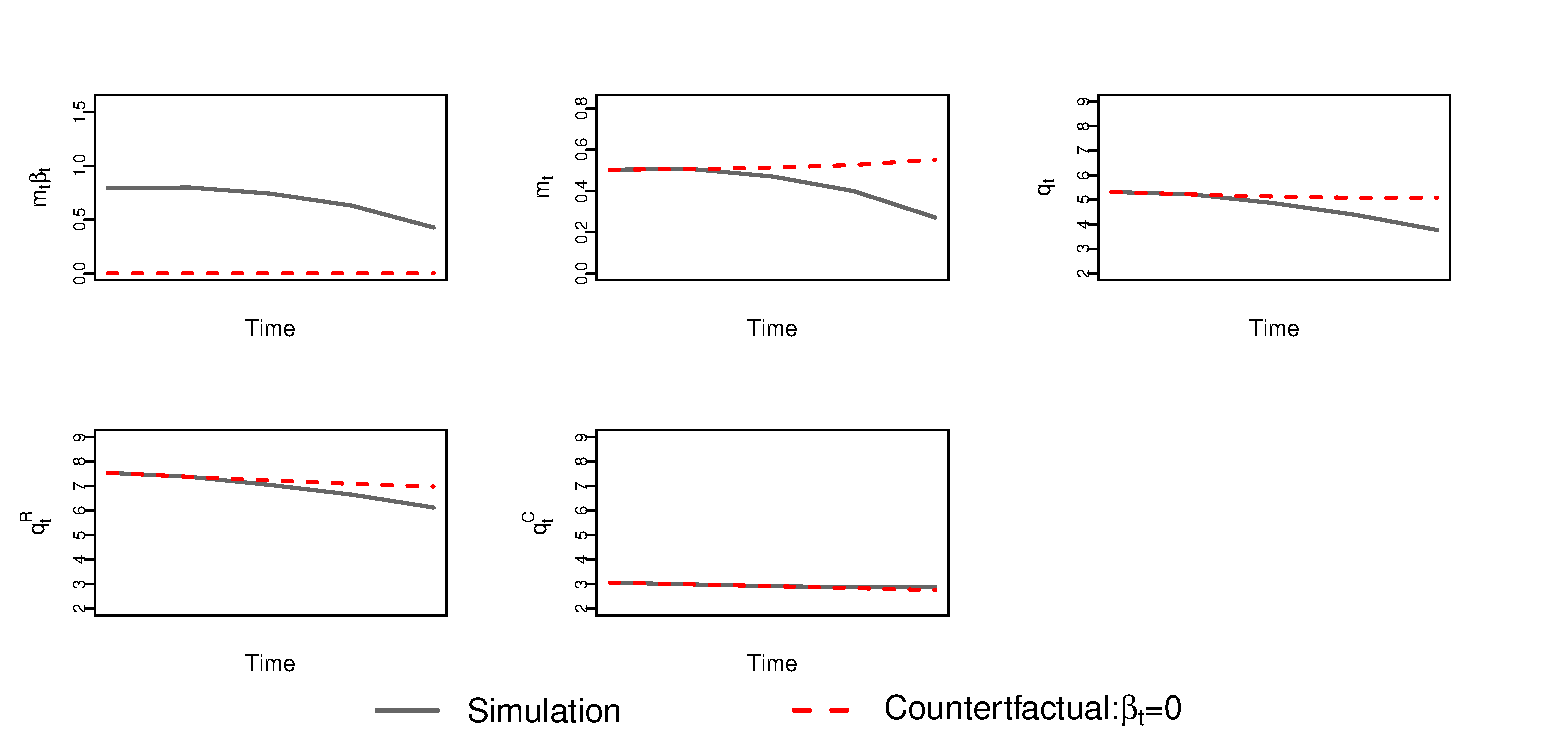
\includegraphics[width=.99\textwidth]{dynamics.pdf}
\caption{Counterfactual Experiment: $\overline{\beta}=0$}
\label{fig:exp}
\end{figure}



\section{Alternative Theories}

\begin{itemize}
\item Out of Italy by Fernand Braudel. \href{https://www.globalpolicyjournal.com/blog/07/08/2020/darkness-illuminated-world-italy-braudel}{summary by Milanovic}	
\end{itemize}

\section{Conclusion}

\section{To do}
\begin{itemize}
\item In the dataset Tito Placido shold be "Titi"+ update info using the index.
\item Non religious censorship. According to Amir Alexander, one of the reason why Galileo was persecuted was becuase of the use of infinitesimal in his math, which was an idea that Jesuits wanted to fight. The use of infinitesimals did not spread in Italy since Jesuits forbit it in their powerful order (kind of self censorship). After Torricelli and Cavalieri, no one in Italy could continue to use this techniques. Instead, in UK the indea of infinitesimals started spreading thanks to John Wallis. Later, Boyle and Newton built on this techniques.	
\item Gingerich found that about two thirds of the copies of \textit{De revolutionibus} in Italy at the time of the decree were "corrected." However, virtually none of the copies outside Italy, among which Spain and France, were touched. \cite{gingerich2004} analyzes 277 copies of the first edition and 324 of the second of \textit{De revolutionibus}.
\end{itemize}	
\section{Comments}
\begin{enumerate}
\item Measuring quality using the number of publications about one author can be due to the fact that people wrote about him because he was censored. If this is the case, the higher quality of censored people might just reflect this fact.
\item Joel comments:

\begin{itemize}

	

\item Some academies had corresponding members. Some of the foreign members of the academy might have never visited Italy: can you check whether they actually spent some time there? Otherwise you might want to check whether your results/ empirical regularities still hold once you drop scholars born abroad.
\item You look at the role of written knowledge, while also tacit knowledge matters. It might be that after censorship has been in place, people shifted to tacit knowledge to avoid censorship.
\item Even thought the Church could control Italian printers, she could not do so for foreign ones. Some of those books might have reached Italy through smuggling. In particular, many books printed in Basel used to enter Italy in this way.
\item You look at scholars based in Italy only. Why? At the time a 'Republic of Letters' was in place: italian scholars could learn heretical ideas from other from northern Europe, where censorship could not be enforced. I can give you examples of that. Moreover, Italian heretical scholars could leave Italy and stay in contact from there with they former colleagues.
\item I am not very convinced by the fact that $ \overline{\beta}$ could be lower than 1. One way to motivate it would be to find examples of books where the heretical part was 'hidden' using metaphors.
\item An interesting experiment would be to set $ \overline{\beta}_{Italy}=\overline{\beta}_{northern europe}$.
\item Your story is about censorship in any field. For censorship in mathematics, read 'Infinitesimal: How a Dangerous Mathematical Theory Shaped the Modern World' by Amir. It is about the aversion of Jesuits on infinitesimal calculus.
\item Other literature related to your research: Feingold 'Jesuit Science and the Republic of Letters'+Eric Chaney on islamic science+Tabellini and Serafinelli
\end{itemize}
\item Jame Fenske comments:
\begin{itemize}
\item It would make more sense if the Church was constrained to Censor a maximum quantity of books. [In the model it is as if the number of book was constant. Maybe in the robustness we can link $ \overline{\beta}$ to the number of editions published in Italy in $t$.]
\item I would expect that the Church looked in particular for high quality heretical guys, rather than sampling from the whole distribution. Then in a second moment she can start censoring the average guy.
\item Literature: see Mark Koyama on Chinese censorship.
\item If you could disentangle the effect of self versus direct censorship it would be nice.
\item Read a lot of books about the historical context to motivate your model assumption: people could think at many ideas different than yours that match the data.
\item If you want to link the censorship capacity to the enforcement of the Church is a region, look at the number of catholic churches in that region or whether who was in power was close to the vatican [mah..].
\item Other measures of quality: whether the book has been "imitated" or cited in the future. Check how Dittamar compute the quality of books.
\end{itemize}
\item Does censorship depends on the field of publication?
\item Sasha Becker comments:
\begin{itemize}
\item The way I see censorship in Italy is more a "Religion versus secularism" thing rather than "revolutionary versus non revolutionary". According to Cantoni (2018) Protestant Reformation caused a reallocation of resources from religious to secular.[We can check censorship by field].
\item You might want to check how thing changes by region. In the Vatican state censorship could be fully enforced, in Venice it depended on the size of business of venetian printers in Rome.
\end{itemize}

\end{enumerate}





\bibliographystyle{achicago}
\bibliography{prohibitorum}

\appendix
%\counterwithin{figure}{section}
%\counterwithin{table}{section}
\section*{Appendix}

\section{Fit of the Model to the Data}\label{appendix:a}
\begin{figure}[htpb]
\centering
\includegraphics[width=.99\textwidth]{fit.pdf}
\caption{Fit of the Structural Model}
\label{fig:fit}
\end{figure}


\begin{figure}[htbp]
\centering
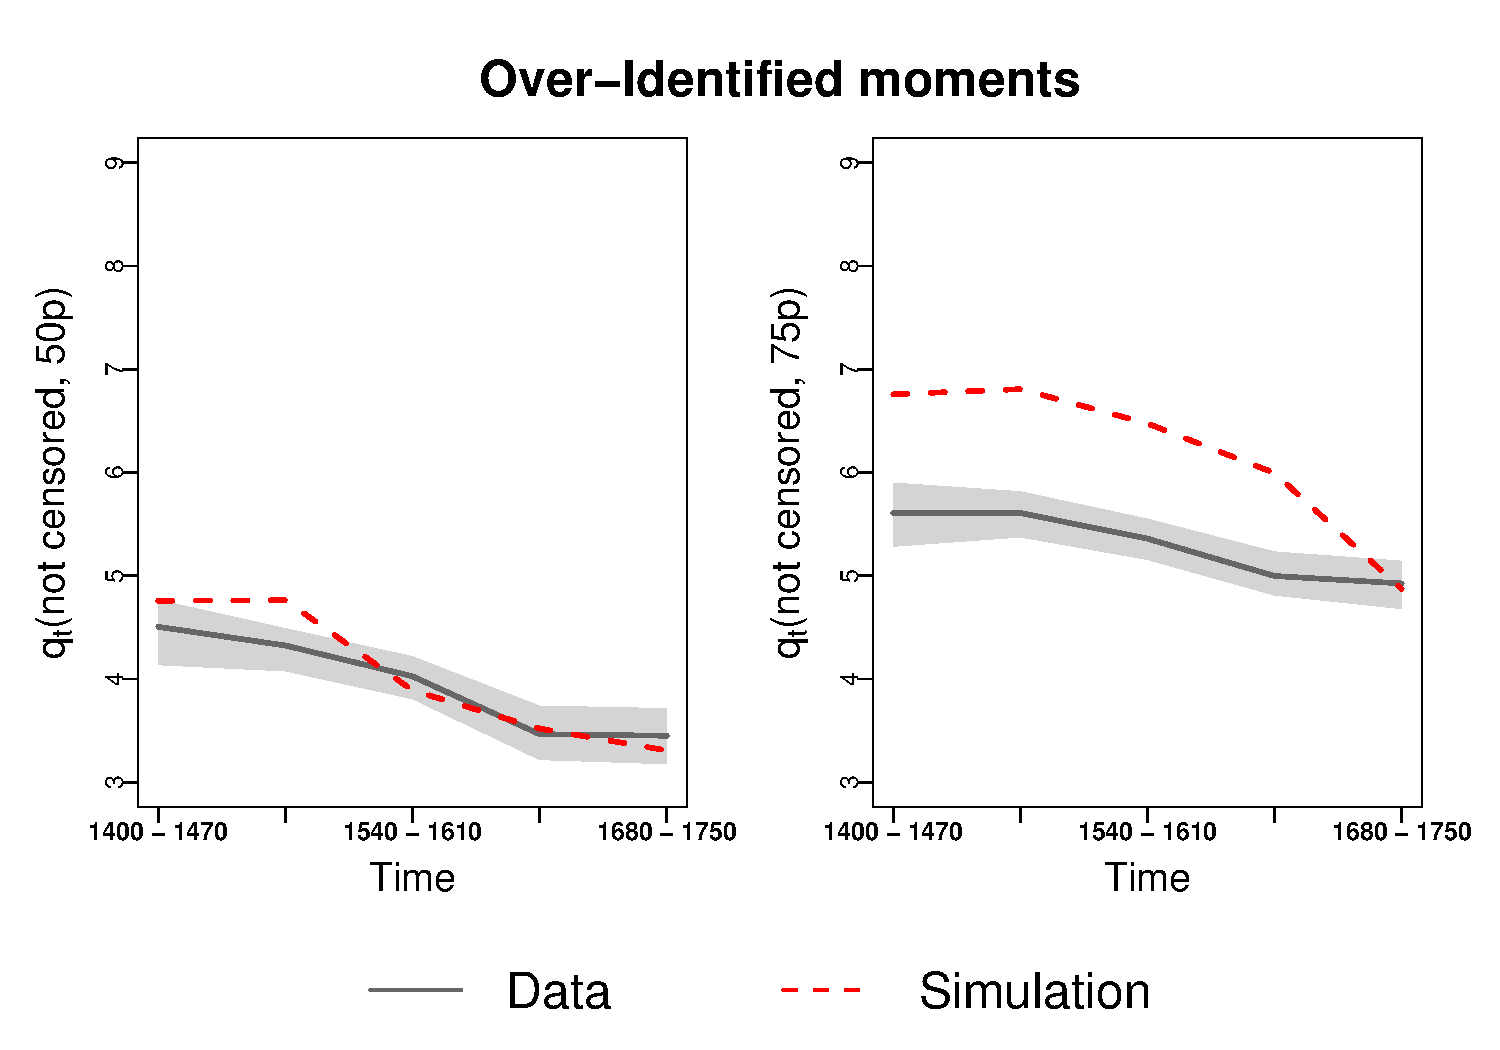
\includegraphics[width=.7\textwidth]{over.pdf}
\caption{Overidentifying Restrictions}
\label{fig:over}
\end{figure}

\FloatBarrier


\section{Accounting for Self-Censorship}\label{appendix:b}
In this section of the appendix we estimate a variation of our model which accounts for self-censorship. As it was described in subsection \ref{subsection:censor}, the only variation is the introduction of the parameter $\gamma$. We have some self censorship when the parameter takes a value lower than 1. The parametrization procedure is similar to the one presented in section \ref{section:identification}: the only differences the introduction of $\gamma$ among the parameters estimated with the method of simulated moments. We allow $\gamma$ to take values above from 0 to over 1: $\gamma$ being above 1 is counter intuitive and it would suggest a probable misspecification of the model.  Results are shown in Table~\ref{table:paramss}. We can notice that the estimated parameters are very close to the ones of the standard model, which are reported in Table~\ref{table:param}, but most importantly $\gamma$ is very close to unity, meaning that self censorship is a feature of secondary importance for understanding the effect of Church's censorship. Moreover, the standard errors of $\gamma$ are large, which makes the parameter not statistically different from 1 at the $90\%$ level, which further supports the idea that self-censorship was not key for the evolution of knowledge. Figures \ref{fig:fits}, \ref{fig:overs} and \ref{fig:exps} respectively show the fit, the over-identifying restrictions and the counterfactual experiment of the self-censorship model. The results are very close to the baseline model.

\begin{table}[htpb]
    \caption{Identification of Parameters}
    \centering % used for centering table
    \begin{tabular}{@{} l c c c @{}}
    \hline%inserts double horizontal lines
     \ Calibrated Parameters &  & Value & Target  \\ [0.05ex] % inserts table
     \hline
     Discount Factor  & $\delta$   &0.5&   RBC literature\\[0.15ex]
     Fixed Cost of Censorship  & $\psi$   &(0.152-0.168)& Censorship start \\[0.15ex]
     \hline % inserts single horizontal line
    \ Estimated Parameters &  & Mean & Standard Errors  \\ [0.05ex] % inserts table
      %heading
    \hline % inserts single horizontal line
    \rule{0pt}{2.5ex}
    Mean quality in 1  & $\overline{q}_1$   & 4.99 & 0.218  \\[0.15ex]
    Mean R quality in 1  & $\overline{q}^R_1$   & 7.05 & 0.349  \\[0.15ex]
     Productivity of books  & $\theta$   & 0.14 &  0.02  \\[0.15ex]
    \ Max Censorship  & $\overline{\beta}$   & 0.15 &  0.027   \\[0.15ex]
    Knowledge growth & $(1+\nu)\mu$   & 1.97 &  0.395   \\[0.15ex]
    Price of revolutionary books   & $p$   & 0.39 &  0.049  \\[0.15ex]
     Self Censorship Parameter   & $\gamma$   & 0.97 &  0.122  \\[0.15ex]
    \hline
    \end{tabular}
    \label{table:paramss}
    \end{table}

\begin{figure}[htbp]
\includegraphics[width=.99\textwidth]{dynamicsss.pdf}
\caption{Counterfactual Experiment: $\overline{\beta}=0$. Model with censorship}
\label{fig:exps}
\end{figure}

\begin{figure}[htpb]
\centering
\includegraphics[width=.7\textwidth]{fitss.pdf}
\caption{Fit of the Structural Model with self-censorship}
\label{fig:fits}
\end{figure}


\begin{figure}[htbp]
\centering
\includegraphics[width=.7\textwidth]{overss.pdf}
\caption{Overidentifying Restrictions with self-censorship}
\label{fig:overs}
\end{figure}

\FloatBarrier


\end{document}

[[[OLD PIECE OF PROOF]: since $\mathcal{D}(0)<0$, $\mathcal{D}(1)<0$ and $\mathcal{D}(m^*)>0$, we can invoke twice the intermediate value theorem to prove that there exist at least one $m'\in[0,m^*]$ and at least one $m''\in[m^*,1]$ such that $\mathcal{D}(m')=\mathcal{D}(m'')=0$.
If $\psi=0$, $\overline{m}=0$, $\hat{m}=1$ and it holds $V^C(m)-\psi>V^N(m)\;\forall\;m\in(\overline{m},\hat{m})$.]]
\subsection{Preferences and Production}
 We consider an economy populated by $N$ agents that live one period and then die with probability one. Time is discrete and goes from $0$ to $\infty$. Individuals care about consumption only: the utility of individual $i$ is given by
\begin{equation}
U(c^i), \quad \text{with} \quad U'>0.
\end{equation}
Agents inelastically supply one unit of labor, whose effectiveness in terms of output depends on the idiosyncratic productivity of the individual, $k^i$.
The consumption good is produced with a constant return to scale Cobb-Douglas technology, whose input are labor $L$ and land $M$
\begin{equation}
Y=L^\alpha M^{1-\alpha}.
\end{equation}
The amount of land stays constant over time and we normalize it to 1. Land is owned by the population, but the way in which land is shared between agents will not affect our results. Now we will be more precise in linking the current stock of knowledge with total production. Individual labor productivity $L_i$ is heterogeneous across agents and equals:
\begin{equation}\label{eq:indout}
L_i=h_i^{-\theta},
\end{equation}
where $h_i$ is an idiosyncratic cost parameter that measures the productivity of the individual: the lower the value of this parameter, the larger the output. The value of $h_i$ represents the idiosyncratic knowledge of each individual, acquired though diffusion of the stock of knowledge left by previous generations: this process will be explained in detail in the next subsection. $h_i$ is drawn from an exponential distribution with scale parameter $k$, which represents the quality of the current stock of knowledge:
\begin{equation*}
h_i\sim \exp(k).
\end{equation*}
Given that its distribution is exponential and given \ref{eq:indout}, the distribution of labor supply follows a Fréchet distribution with scale parameter $k^\theta$ and shape parameter $1/\theta$. This allows us to write the average labor supply $\bar{L}$ as:
\begin{equation}
E(L_i)=\int_0^\infty h^{-\theta}_i (k e^{-k h_i})dh_i=k^{\theta}\Gamma(1-\theta),
\end{equation}
where $\Gamma(x)=\int_0^\infty s^{x-1} e^{-s}ds$ is the Euler gamma function. It follows that total labor supply equals
\begin{equation}
L=N E(L_i)=N k^{\theta} \Gamma(1-\theta).
\end{equation}
\subsection{Knowledge Diffusion and Occupational Choice}
So far we have described how knowledge affects production, but not how the stock of knowledge evolves over time. Also, we did not mention the occupational choice that agents make. In our model there will be two different sectors: a \textit{compliant} one, indicated by the superscript $C$, where the type of knowledge that is used for production is acquiescent with the ideology of the Roman Church,\footnote{Note that being compliant does not necessarily mean to produce using the official Roman Church doctrine as an input: this is true just for the production of religious books or religious services in general. Instead, it just mean that the knowledge should not contradict the Roman Church doctrine.} and a \textit{revolutionary} one, indicated by the superscript $R$, which indicates that the knowledge used for production is considered to be heretical by the Roman Church.
We define $k^R$ the amount of knowledge of the revolutionary sector and  $k^C$ the quality of knowledge in the compliant one. These variables represent a stock of knowledge in the sense that they govern the average productivity by occupational sector:
\begin{equation}
h^j_i \sim \exp(k^j), \quad \text{with} \ j\in \{C,R\} \ \text{and} \ i\in \{1,..,N\}.
\end{equation}
 Note that these two variable also represent the state variables of the economy.
 During their life, individuals acquire knowledge coming from the previous generation\footnote{We can think that the knowledge of the previous generation is embodied in books, objects or other human creations that are transmitted to future generations.}. Every individual encounter $\mu$ ideas during her life, where some of them belong the compliant and other to the revolutionary type. Each individual retains the best idea coming from each one of the two distributions, and will store this knowledge, making it available to future generations. Note also that the number of revolutionary ideas that each agent will encounter in $t$ depends on the the share of individuals that produced with the revolutionary technology in the previous generation, which is denoted by  $m_{t-1}$. Therefore, a individual will meet $\lfloor \mu m_{t-1} \rfloor$ revolutionary ideas  and $\lfloor \mu (1-m_{t-1}) \rfloor$ compliant ideas, draw at random along her life and before she starts producing. Formally, the process of retaining the best ideas by sector is described as
\begin{align*}	
   \hat{h}^C_i&=\text{min}\{h^C_1,..,h^C_{\lfloor(1-m_{t-1}) \mu\rfloor}\}\ \sim \exp(k^C (1-m_{t-1}) \mu),
 \\ \hat{h}^R_i&=\text{min}\{h^R_1,..,h^R_{\lfloor m_{t-1} \mu \rfloor}\}\ \sim \exp(k^R m_{t-1} \mu),
 \end{align*}
where $ \hat{h}^C_i$ is the potential output if $i$ decides to produce using the compliant technology, while she would produce $ \hat{h}^R_i$ using the revolutionary one. Note the distribution of retained ideas maintains the same shape with a different scale parameter, which follows from the property of the exponential distribution. For the sake of simplicity, from now on we will approximate $\lfloor(1-m_{t-1}) \mu\rfloor$ and $\lfloor m_{t-1} \mu \rfloor$ to respectively  $(1-m_{t-1}) \mu$ and $m_{t-1} \mu $, so that we will be able to proceed our analysis treating the number of encountered ideas as a continuous variable. Since both the best revolutionary and compliant ideas are retained and transmitted to the next generation, the aggregate stock of knowledge by type evolves over time according to:
 \begin{align}
  k_{t}^C&=k_{t-1}^C (1-m_{t-1}) \mu,\label{eq:kCtime} \\
  k_{t}^R&=k_{t-1}^R m_{t-1} \label{eq:kRtime} \mu.
 \end{align}

Once the individual has been through the process of retaining the best idea for each type, she will choose whether to use the compliant or the revolutionary idea to produce in the market. We assume that she will choose the one bringing her more consumption, hence the most productive one. It follows that the average productivity is
\begin{equation}
 h_i=\text{min}\{\hat{h}^C,\hat{h}^R\} \ \sim \exp(k^C+k^R)=Exp(k),
\end{equation}
while the probability\footnote{For $N$ big enough we can apply the law of large numbers and say that $m$ is also the share of chosen revolutionary ideas} that the revolutionary idea is chosen is:
\begin{equation}\label{eq:sharer}
m=\text{Prob}\{\hat{h}^C>\hat{h}^R\}=\frac{k^R}{k^R+k^C},
\end{equation}
which follows from the properties of the exponential distribution.

\section{Model Calibration}
What we have both in the data and in the Model:
\begin{itemize}
\item \% Censored books: $m_t \beta$
\item Average output of revolutionary to  non revolutionary ideas (given $\theta$): $z_t^\theta$. $\theta$ can be taken such that the fictional distribution of productivity resembles the one of scholar's quality (Fit a Fréchet distribution to the overall distribution of output quality. I get a shape and a scale parameter which are respectively $1/\theta$ and $k^\theta$ in the model.)
\end{itemize}
Then, distinguishing between the two models:
\begin{itemize}
\item \textit{Rule of Thumb Model}. Assuming that $t=0$ happens when we first observe the data, we can have $\beta$ from \ref{proposition:rthumb} and from the fact of observing $m_0\beta$. A good test for the model would be to see that the $m_0$ that arise from this method and the other one arising from \ref{eq:sharer} coincide. Then, we can let the model work and see if the simulations resembles what happened in the data. PROBLEM: given $m_0\beta=0.1$, using \ref{proposition:rthumb} we get $\beta=0.18$, which seems inconsistent with the observed distribution of the quality of authors (there are almost no top authors that were not censored).
\item \textit{Maximizing model}. Here, the thing that we would like to have is first to have a period with rising $m$ and no censorship, and a second period with a decreasing censorship and a decreasing $m$. PROBLEM: In order to have that, we need $m_0>0.5$ (see \ref{proposition:dynex}) and hence also $\overline{m}>0.5$. Again, given $\overline{m}\overline{\beta}=0.1$, we get $\overline{\beta}<0.2$, , which seems inconsistent with the observed distribution of the quality of authors (there are almost no top authors that were not censored).
One possible solution to this: assuming that revolutionary comes from $\exp(\psi k^R)$ will give as a result that, without censorship, revolutionary ideas start diverging at $1/(1+\psi)$.
\end{itemize}


%Here old proposition, assumption and proofs

From now on we restrict our attention to the region of parameters that allows for the possibility that $m_t$ is first rising and then declining over time.
\begin{assumption}\label{assumption:half}
$V^C(1/2)-\Psi<\frac{u(1/2)}{1-\delta}$.
\end{assumption}
Assumption \ref{assumption:half} tells us that it is optimal not to set up the censorship apparatus when $m_t=1/2$, which is the threshold below which $\lim_{t\to\infty} m_t=0$ even without imposing censorship. In this scenario Proposition \ref{proposition:threshold1} holds:

\begin{proposition}\label{proposition:threshold1}
Under Assumption \ref{assumption:half}, $V^C(m_t)-\Psi<V^N(m_t) \; \forall \; m_t\leq 1/2$.
\end{proposition}
\begin{proof}
See appendix \ref{appendix:a}.
\end{proof}

Proposition \ref{proposition:threshold1} is important because it allow us to claim that the Church will never build a censoring apparatus as soon as the share of revolutionary books will converge naturally to 0. \ref{proposition:threshold1} also imply that, if a threshold $\overline{m}$ for setting up a censoring apparatus exists, it must be that $\overline{m}>1/2$, which allows for a region where the share of revolutionary books is increasing and the Church waits before acting. We need to impose one additional assumption for proving the existence and uniqueness of such threshold:
\begin{assumption}\label{assumption:inf}
Defined $\overline{m}=1/(2-\overline{\beta})$, $\forall\;m'\geq\overline{m}$ it holds that $V^C(m')=-\infty$. [I would like this to follow from preferences. From this it follows that the Church NEVER choose an equilibrium path that leads asymptotically to $m_t=1$.]
\end{assumption}
Assumption \ref{assumption:inf} assures that the Church, if she has the possibility, she will never take an action that will leads to a revolutionary steady state. This additional assumption turns out to be crucial for the existence and uniqueness of the threshold.
\begin{proposition}\label{proposition:threshold}
Under assumptions \ref{assumption:half} and \ref{assumption:inf}, $\exists! $ $\overline{m}\in(1/2,1/(2-\overline{\beta})]$ such that $V^C(\overline{m})-\Psi=V^N(\overline{m})$. Moreover, it holds:
\begin{itemize}
\item Proposition \ref{proposition:conv} holds.
\item If a censorship apparatus has not been established yet, it will if and only if $m_t\geq\overline{m}$.
\end{itemize}
\end{proposition}

\begin{proof}
To be done.
\end{proof}


%Proofs that were in the appendix
\begin{proof} of Proposition \ref{proposition:threshold1}.\\
First, we define $\hat{V}^N(m_t)$ the value function of the Church if she never switches to a censorship regime and note that $\hat{V}^N(m_t)\leq V^N(m_t)\;\forall\;m_t$. Now, let's define $\mathcal{D}(m_t)=\hat{V}^N(m_t)-V^C(m_t)+\psi$, which can be written as
\[
\mathcal{D}(m_t)=\sum_{s=t}^{\infty}\delta^s\log\bigg[\frac{-1}{-(\frac{m_t}{1-m_t})^{2^s}-1}\bigg]-\delta^s\log\bigg[\frac{-1+\overline{\beta}}{-(\frac{m_t}{1-m_t}\overline{\beta})^{2^s}-1+\overline{\beta}}\bigg]=\sum_{s=t}^{\infty}\delta^s time_s(m_t)
\]
Now note that $time_s(m_t)$ is decreasing in $m_t$
\[
\frac{\partial time_s(m_t)}{\partial m_t}=\frac{2^s \left(\frac{\overline{\beta} -1}{\beta -\left(\frac{(\overline{\beta} -1) m_t}{m_t-1}\right)^{2^s}-1}-\frac{1}{\left(\frac{m_t}{1-m_t}\right)^{2^s}+1}\right)}{(m_t-1) m_t}\leq0
\]
from which it follows directly that also $\frac{\mathcal{D}(m_t)}{\partial m_t}\leq0$. Now note that since 0 is a stable steady states of the dynamics of $m_t$ as Proposition \ref{proposition:dynex} states, we can write $\mathcal{D}(0)=\hat{V}^N(0)-V^C(0)+\psi=\psi$. Now, since $\mathcal{D}(m_t)$ is non increasing, $\mathcal{D}(0)>0$ and $\mathcal{D}(1/2)>0$ from Assumption \ref{assumption:half}, we can conclude that for $m_t\in[0,1/2]$ we have $\hat{V}^N(m_t)>V^C(m_t)-\psi$. Since $\hat{V}^N(m_t)\leq V^N(m_t)\;\forall m_t$, then it also holds $V^N(m_t)>V^C(m_t)-\psi$ for $m_t\in[0,1/2]$.
\end{proof}

\begin{proof} of Proposition \ref{proposition:threshold}.\\
Before we start the proof, we will refer to $m_t^+$ and $m_t^-$ to the $m_t$ that is obtained applying \ref{eq:lawm} forward and backward when $\beta=\overline{\beta}$. Similarly, we will refer to $f^{+1}(m_t)$ and $f^{-1}(m_t)$ to the $m_t$ that is obtained applying \ref{eq:lawm} forward and backward when $\beta=0$.
\textbf{Existence.} Firstly, notice that if a threshold $\overline{m}$ exists, it cannot be $\overline{m}\leq 1/2$ because of Proposition \ref{proposition:threshold1}, and it cannot be $\overline{m}>f^{-1}(1/(2-\overline{\beta}))$ because of Assumption \ref{assumption:inf}.
We define $\mathcal{D}(m_t)=V^C(1/2)-\psi-V^N(1/2)$, which is a continuous function in $[1/2,f^{-1}(1/(2-\overline{\beta})]$ because $V^C$ and $V^N$ are. Moreover, $\mathcal{D}(1/2)<0$ and $\mathcal{D}(f^{-1}(1/(2-\overline{\beta}))>0$  because $V^C(1/2)-\psi<V^N(1/2)$ and $V^C(f^{-1}(1/(2-\overline{\beta}))-\psi<V^N(f^{-1}(1/(2-\overline{\beta}))$. We can now invoke the intermediate value theorem to prove that there exists at least one value of $m_t$ such that $\mathcal{D}(m_t)=0$ in $[1/2,f^{-1}(1/(2-\overline{\beta})]$. This also imply that there exists at least one value of $m_t$ such that $V^C(m_t)-\psi=V^N(m_t)$.\\
\textbf{Uniqueness.} We prove uniqueness by contradiction. Suppose that exist two thresholds $m_L$ and $m_H$ with $m_H>m_L$ such that $V^C(m_L)-\psi=V^N(m_L)$ and $V^C(m_H)-\psi=V^N(m_H)$. Note that it holds $V^C(m)-\psi\geq V^N(m)$ for $m\geq m_H$ and $V^C(m')-\psi\leq V^N(m')$ for $m_L\leq m'\leq m_H$ because of the continuity of the two functions and because of Assumption \ref{assumption:inf}. Now, suppose it holds $m_L^+\leq m_H$, which implies
\begin{multline*}
\log(1+m_L)+\delta V^C(m_L^+)-\psi\delta>\log(1+m_L)+\delta V^C(m_L^+)-\psi\\=V^C(m_L)-\psi=V^N(m_L)=\log(1+m_L)+\delta V^N(m_L^+).
\end{multline*}

This leads to a contradiction because it cannot be that $m_L^+\leq m_H$ and $V^C(m_L^+)-\psi>V^N(m_L^+)$ hold at the same time.

Now, suppose instead that $m_L^+> m_H$ hold. Then:
\[
\log(1+m_L)+\delta V^C(m_L^+)-\psi=V^C(m_L)-\psi=V^N(m_L)=\log(1+m_L)+\delta (V^C(m_L^+)-\psi),
\]
which simplified gives
\[
\psi=\delta\psi,
\]
which again is a contradiction for $\psi>0$ and $\delta<1$.\\
\textbf{Dynamics.} That the censorship apparatus will be established if and only if $m_t\geq\overline{m}$ follows trivially from the proof of existence and uniqueness. Instead, the dynamics of Proposition \ref{proposition:dynex} hold
\end{proof} 